\documentclass[11pt, a4paper, titlepage]{article}
\usepackage[left=2cm, right=2cm, top=2cm, bottom=2cm]{geometry}
\usepackage[style=authoryear,dashed=false,backend=bibtex]{biblatex}
\bibliography{MiniProject}
\usepackage{graphicx}
\usepackage{lineno}
\usepackage{csvsimple}
\usepackage{datatool}
\linespread{1.5}

\newcommand\wordcount{\documentclass[11pt, a4paper, titlepage]{article}
\usepackage[left=2cm, right=2cm, top=2cm, bottom=2cm]{geometry}
\usepackage[style=authoryear,dashed=false,backend=bibtex]{biblatex}
\bibliography{MiniProject}
\usepackage{graphicx}
\usepackage{lineno}
\usepackage{csvsimple}
\usepackage{datatool}
\linespread{1.5}

\newcommand\wordcount{\documentclass[11pt, a4paper, titlepage]{article}
\usepackage[left=2cm, right=2cm, top=2cm, bottom=2cm]{geometry}
\usepackage[style=authoryear,dashed=false,backend=bibtex]{biblatex}
\bibliography{MiniProject}
\usepackage{graphicx}
\usepackage{lineno}
\usepackage{csvsimple}
\usepackage{datatool}
\linespread{1.5}

\newcommand\wordcount{\documentclass[11pt, a4paper, titlepage]{article}
\usepackage[left=2cm, right=2cm, top=2cm, bottom=2cm]{geometry}
\usepackage[style=authoryear,dashed=false,backend=bibtex]{biblatex}
\bibliography{MiniProject}
\usepackage{graphicx}
\usepackage{lineno}
\usepackage{csvsimple}
\usepackage{datatool}
\linespread{1.5}

\newcommand\wordcount{\input{MiniProject.sum}}

\begin{document}

\begin{titlepage} % Suppresses headers and footers on the title page
	
	\centering % Centre everything on the title page
	
	\scshape % Use small caps for all text on the title page
	
	\vspace*{\baselineskip} % White space at the top of the page
	
	%------------------------------------------------
	
	%	Title
	
	%------------------------------------------------
	
	\rule{\textwidth}{1.6pt}\vspace*{-\baselineskip}\vspace*{2pt} % Thick horizontal rule
	
	\rule{\textwidth}{0.4pt} % Thin horizontal rule
	
	\vspace{0.75\baselineskip} % Whitespace above the title
	
	{\LARGE A comparison of a phenomenological model with Holling's mechanistic models for functional responses, focusing on filter and non-filter consumer feeding modes\\} % Title
	
	\vspace{0.75\baselineskip} % Whitespace below the title
	
	\rule{\textwidth}{0.4pt}\vspace*{-\baselineskip}\vspace{3.2pt} % Thin horizontal rule
	
	\rule{\textwidth}{1.6pt} % Thick horizontal rule
	
	\vspace{2\baselineskip} % Whitespace after the title block
	
	%------------------------------------------------
	
	%	Subtitle
	
	%------------------------------------------------
	
	Computational Methods in Ecology and Evolution MRes
	\vspace{0.5\baselineskip}
	
	 MiniProject % Subtitle or further description
	
	\vspace*{3\baselineskip} % Whitespace under the subtitle
	
	%------------------------------------------------
	
	%	Editor(s)
	
	%------------------------------------------------
	
	\vspace{0.5\baselineskip} % Whitespace before the editors
	
	{\scshape\Large Lucy Goodyear\\
		Department of life Sceinces \\
		Imperial College London\\} % Editor list
	
	\textit{lucy.goodyear19@imperial.ac.uk}
	\date{}
	
	\vspace*{3\baselineskip} % Whitespace under the subtitle
	
	Word Count: \wordcount
	
\end{titlepage}
	
\section*{Abstract}
Functional responses, the relationship between a consumption rate and resource density, can be categorised into three types. The first, the type I response, is a linear relationship, exhibited by some filter feeders. The second, the type II response, also known as the Holling Model or the basic functional response, is the most common and represents a response with a non-zero handling time. The third, the type III response, is the generalised functional response, from which the other two can be produced, and is linked to predator switching and learning. All three are examples of a mechanistic model, which is a model based on biological principles. In this paper, the type III response (the generalised functional response), and by extension the other two types, are compared against a phenomenological model, a polynomial, and shown to be a significantly better fit to empirical data. This provides evidence for the outperformance of mechanistic models over phenomenological models. 

Those datasets that were fitted best by the generalised functional response were then subsetted into the three different functional response types in order to identify those best fitted by the Holling type I model. By reviewing these datasets in terms of feeding mode, the claim by Jeschke et al. in their 2004 paper that "type I functional responses are exclusive to filter feeders" is tested and contradicting data is found. This does not conclusively reject the claim, as there are many other factors that could have influenced this result, but rather suggests further study should be done in this area.

\newpage

\linenumbers


%%%%%%%%%%%%%%%% INTRODUCTION %%%%%%%%%%%%%%%%


\section{Introduction}
The term functional response refers to the relationship between a consumer's consumption rate and the density of its prey \parencite{Solomon1949}.  The first mechanistic mathematical approach to functional responses was conducted by Holling in 1959 \parencite{Holling1959b}. Holling constructed an artificial functional response experiment and discovered that the consumption rate is related to prey in terms of two constants: instantaneous rate of discovery and handling time. The instantaneous rate of discovery corresponds to the likelihood of a predator finding an individual prey, expressed as the volume or area searched per unit of time.
The handling time is any time not spent in actively searching for prey. There have been discussions on the different physical activities that handling time includes, such as digestion, time spent consuming prey, time spent hunting prey etc. \parencite{Jeschke2002, Holling1966} but for the purposes of this paper, we are assuming handling time is time spent on any non-foraging activities.
This functional response is the most common in nature and is known as the basic functional response \parencite{Holling1959b}.

In an earlier paper of the same year, Holling describes the shapes of the three functional responses \parencite{Holling1959a} where his experimentally dervied basic functional response can be seen to describe a type II functional response.

Other attempts at modelling functional responses have been made using different assumptions and mathematics; these are discussed by Holling in a later paper, in which he remarks on the lack of biological context in most of the other options \parencite{Holling1965}. Since then, further models have been formalised and changes made to the original Holling equations but these were not used in this paper's hypothesis and  will only be considered in the discussion. 

\bigskip

The type III functional response was modelled using computer simulations and labelled as the generalised functional response by Holling in a later paper \parencite{Holling1965}, with types I and II being limiting conditions. However, type III was not described mathematically until 1977 by Real, who derived it using Holling's type II functional response equation and first-order kinetic interactions \parencite{Real1977}.
 
The generalised functional response equation is written below, where $c$ is the consumer consumption rate, $a$ is the instantaneous rate of discovery, $x$ is the resource density, $h$ is the handling time and $q$ is a variable with as yet unknown biological meaning. It has been hypothesised that $q$ could be related to predator learning and is `the number of encounters...a predator must have with a prey item before becoming maximally efficient at utilizing the prey item as a resource' \parencite{Real1977}.

\begin{equation}
c = \frac{ax_R^{q + 1}}{1 + hax_R^{q + 1}}
\end{equation}

\bigskip

It can be shown that the type II functional response is a special case of the generalised functional response by setting $q = 0$. In terms of Real's interpretation of $q$, this means that the predator `is always maximally efficient on the prey item'  \parencite{Real1977} in a type II response.

\begin{equation}
c = \frac{ax_R}{1 + hax_R}
\end{equation}

\bigskip

 In type I, the handling time is negligible, reducing the second term in the denominator to almost zero, leaving us with a linear relationship:

\begin{equation}
c = ax_R
\end{equation}

Type I responses are to be found in filter feeders, where the predation rate is directly  proportional to the prey density \parencite{Jeschke2004}. This is because filter feeders are able to do activities simultaneously so can effectively spend all their time foraging. There is normally a hard cut-off at very high prey densities, indicating a maximum number of prey that can be caught. \parencite{Jeschke2004}. 

This paper aims to look at whether the generalised functional response equation (a mechanistic model) or a polynomial (a phenomenological model) fits best to empirical functional response data. The polynomial has no biological meaning, so the comparison is effectively one of phenomenological vs mechanistic models. The null hypothesis is that the mechanistic model is no better than a phenomenological model and so the data will be best fit by each model roughly half the time.

By fitting both the general functional response model and a polynomial to 295 empirical datasets, the proportion of best fits by model can be compared. The functional response types were also compared by subsetting by the limiting conditions of type I and type II functional responses, i.e. filtering by the values of $h$ and $q$ respectively, gaining information on the split between the three types. The data can then be subsetted by different metadata fields, such as habitat, in order to look for model fitting trends.

The second part of this paper focusses on the functional response of  filter feeders. In previous work, it has been shown that, although the majority of filter feeders do not show a type I response, the type I reponse is only possible for filter feeders \parencite{Jeschke2004}.  Type I functional responses are characterised by two main conditions: handling time must be negligible and the consumer must always spend the maximal time and effort foraging, the only exception being once the gut is full (satiation condition) \parencite{Jeschke2002}. Many filter feeders have a negligible handing time because they are able to catch prey at the same time as performing other activities, resulting in effectively all of their time being spent foraging. Some filter feeders also adhere to the satiation condition but not many. Both conditions must be met in order for the functional response to be type I, but both conditions could also be met when the resulting functional response is of a different type. This is why it is claimed that the majority of filter feeders (and all non-filter feeders) do not show a type 1 response \parencite{Jeschke2004, Deville2013, Porter1983}. Here, the exclusivity of a type I response to filter feeders is explored in terms of Real's definition of $q$ and derivation of the type III functional response, looking at functional responses when $q$ is not confined to any limits \parencite{Real1977}.  It is expected that there will be full adherence to the paper of Jeschke et al. and so no Holling type I responses are expected to best fit any non-filter feeders.


%%%%%%%%%%%%%%%%%% METHODS %%%%%%%%%%%%%%%%%%%


\section{Methods}

\subsection{Data}

The dataset used is a collection of 4507 records, grouped into 308 IDs, each of which corresponds to a different functional response. The data have been collected from various lab and field experiments, conducted globally, and measure the rate of consumption of a single resource by a consumer, along with various metadata, such as habitat and taxa. There are 68 fields but only 11 have been considered in this paper: ID, consumption rate and resource denisity for fitting the models; consumer foraging movement, resource foraging movement, habitat, experimental conditions (lab/field/enclosure), resource movement dimensionality, consumer movement dimensionality, resource thermal type and consumer thermal type for subsetting the data and looking for trends.

\subsection{Computing Tools}

\subsubsection{Data preparation—R}

Data was prepared for fitting using R v.3.6.1 \parencite{R} because of the ease of viewing data and of accessing and manipulating dataframes. First, the data is subsetted by the necessary columns, all records with missing consumption rates and all IDs with fewer than 5 records are removed (to reduce the possibility of overfitting), which leaves 295 IDs remaining. The data preparation script then generates initial starting values for $a$ and $h$ for the general functional response fit. A new dataframe, including subsetted data and initial starting values for $a$ and $h$, is saved to a csv file.

\subsubsection{Model Fitting — Python}
The starting value optimisation and fitting script is done using Python v.3.7.4 \parencite{Python}. For the polynomial fit, there is an in-built Python function, which also calculates starting values and fit statistics. For the general functional response fit, a Gaussian sample of 6 (chosen for speed of programme execution) is generated around the estimated starting values and each combinatiom of these sample values is used to fit a model to the dataset, resulting in 36 different fits. The AIC, BIC and residual sums of squares (RSS) are calculated for each ID and the starting values for the model with the lowest AIC are chosen as the best fit \parencite{Johnson2004}.  These calculations are perfomed for each ID using parallelisation and the best fit parameters and statsitics are stored in a new dataframe and then saved as a csv for importing into R for the plotting and analysis script.

Functions are saved in a separate Python script and have been generalised to allow importing into future programmes. Two inbuilt Python packages have been used: itertools to try all combinations of the start values, and multiprocessing to allow parallelisation \parencite{Python}. The packages lmfit \parencite{lmfit} v.0.9.14, NumPy \parencite{NumPy} v.1.18.1 and pandas \parencite{pandas} v.0.24.2 were used. NumPy contains the polynomial fitting function as well as different mathematical values, such as $\pi$. The package lmfit allows the use of parameters when fitting a model and pandas is a dataframe tool.

\subsubsection{Plotting and Analysis — R}
The plotting and analysis script has been written in R due to the ease of graphical representation in RStudio and statistical functionality. Four packages are used: ggplot2 \parencite{ggplot2} for visualisation; tidyverse \parencite{tidyverse} for easy data manipulation; DescTools {\parencite{DescTools}}  for stastical tests; and janitor \parencite{janitor} to create flexible tables. After reviewing the datasets, those IDs which haven't been fitted properly are discarded. Some of the inaccurately fitted datasets have a large number of points at very low x-values and then a few at very high x-values, a logarithmic transformation could have been performed on these prior to fitting, but this option was discarded in favour of maintaining the biological significance of $a$ and $h$. This left 280 IDs remaining for analysis.

The script compares RSS, AIC and BIC for each model within each ID and chooses the best fit model based on at least two out of three agreements between these statstics. RSS is used as-is instead of calculating $R^{2}$ due to the new numerous pitfalls in calculating this statistic for non-linear regressions \parencite{kvalseth1985}.
AIC and BIC were chosen because they are the currently viewed as the most appropriate best-fit statsitics \parencite{Johnson2004}. The spread of best fits was compared graphically and a measure of the significance of the resulting proportion of fits between the phenomenological and the mechanistic model was obtained by performing both a G-test of goodness-of-fit and a chi-square goodness-of-fit test. 

The data is then subsetted into the three Holling types by setting any ID with the generalised fucntional response as best fit and $-0.3<q<0.3$ as Holling type II, and any Holling type II with $h<0.1$ as Holling type I. Given $q$ is given no limits in the fitting script, $0.3$ was chosen as the limiting boundary for $q$ visually, based on the whether the resulting plots exhibited a Holling type II or Holling type I shape.
Plots and tables of eight different metadata fields and a table showing the proportion of best fit models in terms of feeding mode are then generated and a G-test of goodness-of-fit is performed to test the significance of the proportion of non-filter feeders best fitted by a Holling type I response.

\subsubsection{Run Script — Bash}

Bash was chosen to join the above scripts into a clear, reproducible workflow because it can run R and Python scripts simply and easily, as well as compile latex files with references.


%%%%%%%%%%%%%%%%% RESULTS %%%%%%%%%%%%%%%%%%%


\section{Results}

\subsection{Mechanistic vs Phenomenological Models}

The findings of a comparison between the mechanistic model and the phenomenological models are shown in Figure 1. It is clear that the mechanistic models are a much better fit. 95.4\% of the data was best fitted by the mechanstic model, which accounts for 267 of 280 IDs. This is highly significtant ($p < 2.2\times10^{-16}$ for both G-test of goodness-of-fit and chi-square goodness-of-fit test), showing that the Holling mechanstic models fit empirical data much better than a polynomial.

\begin{figure}[ht!]
	\centering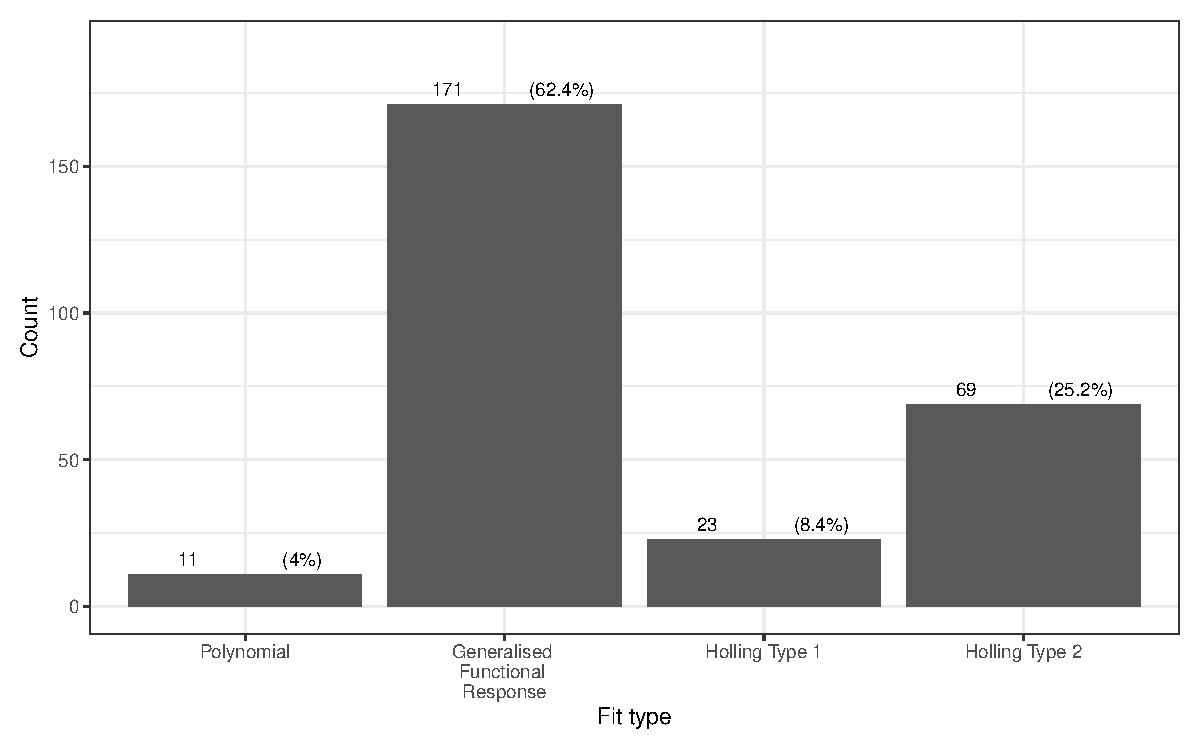
\includegraphics[width=1\textwidth]{../Results/Model_Comparison_Barchart.pdf}
	\caption{ID count by best fit model type}
\end{figure}

\subsection{Data subsets}

The dataset was preliminarily plotted in terms of eight factors: habitat, expermental conditions (lab/field/enclosure), consumer and rescoure thermal type, consumer and resource foraging movement and consumer and resource movement dimensionalty. All of these had a very similar ratio between the different best fits to that of the whole dataset, as can be seen from the four examples in Table 1. The few factors with slightly more varied proportions can be explained by the low quantity of data for that trait, for example passive resource foraging movement, which has only seven records. No particular trait was best fitted by a particular model, which is why the second focus of this paper is filter feeders. 

\begin{table}[ht!]
	\centering\csvreader[
	respect all,
	autotabular
	]{../Results/habitat_table.csv}{}{\csvlinetotablerow}
\end{table}

\begin{table}[ht!]
	\centering\csvreader[
	respect all,
	autotabular,
	]{../Results/labfield_table.csv}{}{\csvlinetotablerow}
\end{table}

\begin{table}[ht!]
	\centering\csvreader[
	respect all,
	autotabular
	]{../Results/res_movement_table.csv}{}{\csvlinetotablerow}
\end{table}

\begin{table}[ht!]
	\centering\csvreader[
	respect all,
	autotabular
	]{../Results/con_movement_table.csv}{}{\csvlinetotablerow}
	\caption{Different fit proportions in terms of various factors. The fit proportions shown by the overall data are shown at the bottom of each table.}
\end{table}

\subsection{Feeding mode}

Each of the IDs best fitted by a Holling type I response was allocated a feeding mode (either filter feeder or non-filter feeder), with the aim of exploring the 2004 claim by Jeschke et al.\parencite{Jeschke2004} that only filter feeders can display a Holling type I functional response. This allocation, along with the reference, can be seen in Table 2 and has been done according to the defintion of a filter feeder in the 2004 paper by Jeschke et al. This is a very broad definition that includes suspension feeders, trap builders, sediment filter feeders, those that only filter feed at certain stages in their lifecycle and also those that change feeding strategies according to prey abundance \parencite{Jeschke2004}.
From Table 2, it is apparent that a total of 11 of the 15 IDs best fit by a Holling type I functional response are classed as non-filter feeders.
This result is not insignifcant ($p < 2.2\times10^{-16}$ using G goodness of fit test). Figure 2 shows an example of a clearly linear functional response for a non-filter feeder consumer that is best fitted by the Holling type I equation.

\begin{table}[h!]
	\small
	\begin{tabular} {| l | l | l |}  \hline
		\textbf{ID} & \textbf{Taxa and Lifestage} & \textbf{Feeding Mode with Reference} \\ \hline
		695 & Stethorus punctum (Adult) & Non-Filter Feeder \parencite{Stethorus}  \\ \hline
		39839 & Rhyacophila dorsalis (Second Instar) &  Non-Filter Feeder \parencite{Rhyacophila}  \\ \hline
		39866 & Notonecta maculata (Fourth instar) & Non-Filter Feeder \parencite{Notonecta}  \\ \hline
		39890 & Anomalagrion hastatum  (Final Instar) &  Non-Filter Feeder \parencite{Anomalagrion}  \\ \hline
		39896, 39905 & Chaoborus americanus ( Fourth instar) & Non-Filter Feeder  \parencite{Chaoborus}  \\ \hline
		39920 & Ranatra dispar (Fifth instar)  &  Non-Filter Feeder \parencite{Ranatra}  \\ \hline
		40010 & Nereis (Hediste) diversicolor (Adult) & Filter Feeder \parencite{Nereis}  \\ \hline
		40019 & Parabroteas sarsi (Adult) & Filter Feeder \parencite{Copepod}  \\ \hline
		40026 &  Cyclops kolensis (Adult) & Non-Filter Feeder \parencite{Cyclops}  \\ \hline
		40066 & Praunus flexuosus (Adult) & Filter Feeder \parencite{Praunus}  \\ \hline
		40089, 40094, 40097 & Sander vitreus (Juvenile) &  Non-Filter Feeder \parencite{Sander}  \\ \hline
		400121 & Aurelia aurita (Juvenile) & Filter Feeder \parencite{Aurelia} \\ \hline
	\end{tabular}
	\caption{The consumers of functional responses best fit by a Holling Type I fit. Feeding mode has been based on the defintion used by Jeschke et al \parencite{Jeschke2004}}
\end{table}

\begin{figure}[ht!]
	\centering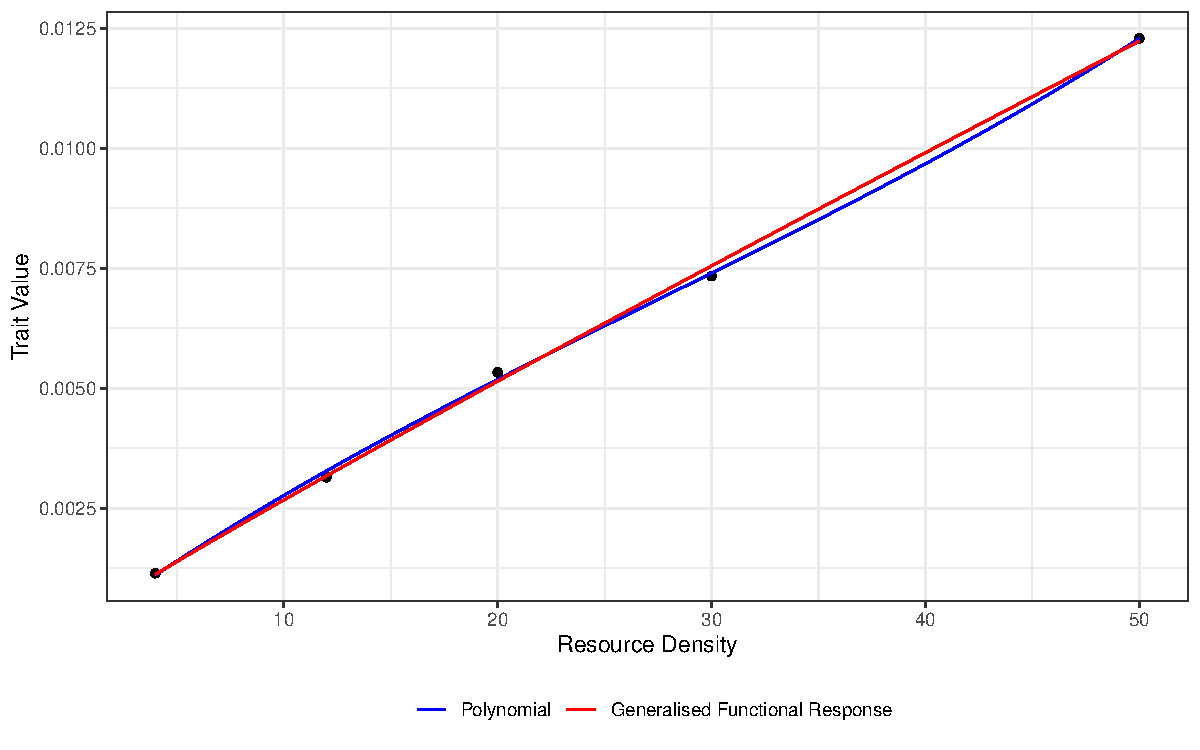
\includegraphics[width=1\textwidth]{../Results/Holling1_example.pdf}
	\caption{Functional response for a non-filter feeder consumer with Holling I best fit (ID = 39920, $q = -.0.055$, $h = 0$)}
\end{figure}


%%%%%%%%%%%%%%%% DISCUSSION %%%%%%%%%%%%%%%%


\section{Discussion}

\subsection{Mechanistic vs Phenomenological Models}

Functional response data are much better explained by the Holling mechanistic models than by a polynomial. This was to be expected, since the parameters in a polynomial do not correspond to biologically meaningful attributes and therefore have no underpinning scientific reasoning.
This is not to say that another mechanistic model might not describe the functional response with even more accuracy; however it does show the value of having models with a biological basis and provides evidence for their outperforming of phenomenological models.

\subsection{The Holling type I response}

The discrepancy between the expected and observed numbers of non-filter feeders with a type I functional response could be explained in two ways:

1) The limiting values of $a$ and $h$ used to subset the Holling type I response from the generalised functional response could have been inadequate, as they were not chosen using a mathematical method. As well as some functional responses being mis-classified as type I, some functional responses that should have been type I may have been missed.

2) Both Holling type II and III functional responses are linear away from the prey density limits. It is possible that not enough data were collected at very low and very high prey densities to display a type II or type III functional response, which is why they have been interpretted as type I.

Several different models have now been produced and  further work has been done to refine the Holling models, with modifications to account for both predator and prey size \parencite{Aljetlawi2004}, foraging dimensionality \parencite{Pawar2012} and changes over spatial scales \parencite{Rincon2017}, among others, all of which could impact the results of this study. The work by Seo and DeAngelis in describing the type I response shows a much more complicated dynamical system than formerly hypothesised \parencite{Seo2011}, which, if considered in this paper, could have provided evidence for the type I exclusivity to filter feeders. Many different models could further be applied to the empirical dataset to better understand the functional responses of both filter and non-filter feeders.

\subsection{The Holling type II and type III responses}

Although not an interest of this paper, it is worth noting the high proportion of IDs with a type III response as the best fit, given that type II is considered to be the most common generally \parencite{Holling1959b}. This is most likely explained by the strict boundaries imposed between the two types. The fitting and tests done in this paper do not reflect the complexities of the two types or the overlaps that are commonly seen. If the plots of those IDs classed as type III are viewed, it can be seen that many better resemble a type II curve ( an example ID is shown in figure 3), suggesting further differentiation is needed than just setting $q\approx0$. This could be because this work has not taken into account intermediate functional responses, which may better explain much of the dataset than the pure repsonses \parencite{Jeschke2004}.

\begin{figure}[ht!]
	\centering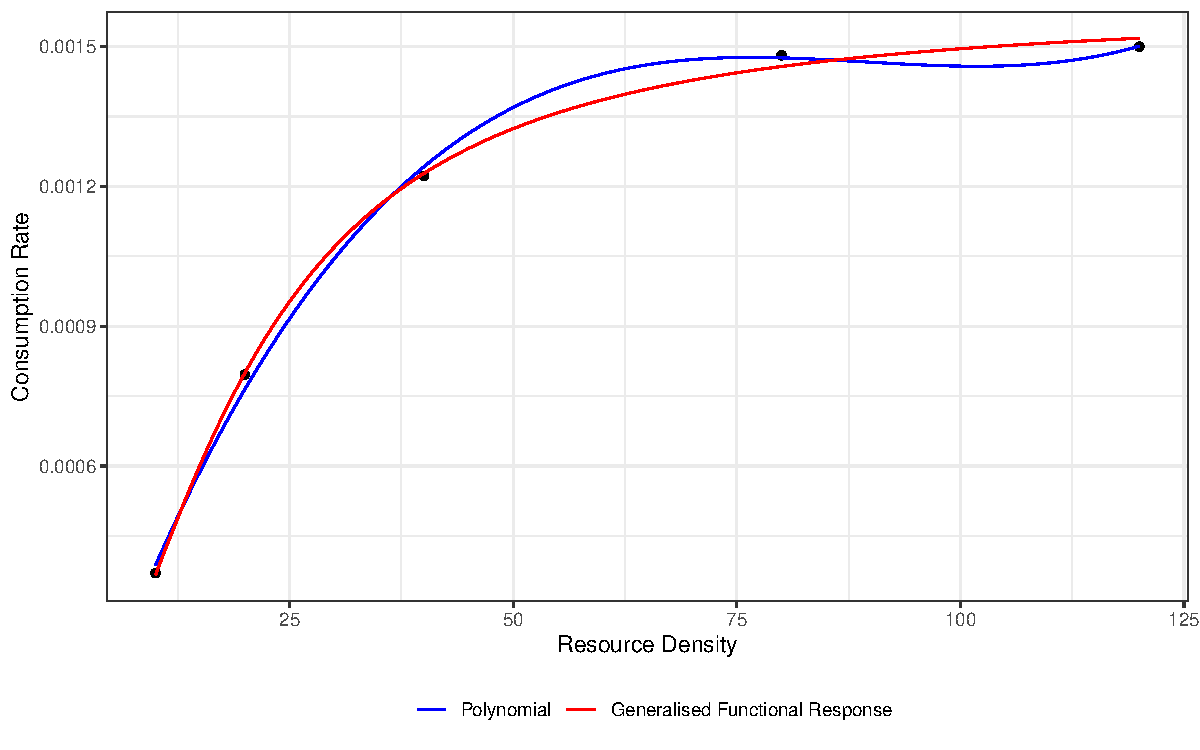
\includegraphics[width=1\textwidth]{../Results/GFR_Holling2_example.pdf}
	\caption{Holling Type II shape for a functional respnse best fit by a general functional response equation (ID = 39864, $q = 0.764$, $h = 632$)}
\end{figure}

\subsection{Concluding Remarks}

In the case of the Holling models and a polynomial, mechanistic models fit significantly better to an empirical dataset than phenomenological models. Although this might not be true for all mechanistic models as it depends on the accuracy of the model in describing nature, this is strong evidence for the superiority of mechanistic models over phenomenologial models.

Within the limits of the data provided, a Holling type I response is not exclusive to filter feeders, as has been previously suggested. However this may be due to a number of factors and so further research is required, perhaps using more sophisticated versions of Holling's models, to gain a more accurate picture.


\newpage
\printbibliography

\end{document}
}

\begin{document}

\begin{titlepage} % Suppresses headers and footers on the title page
	
	\centering % Centre everything on the title page
	
	\scshape % Use small caps for all text on the title page
	
	\vspace*{\baselineskip} % White space at the top of the page
	
	%------------------------------------------------
	
	%	Title
	
	%------------------------------------------------
	
	\rule{\textwidth}{1.6pt}\vspace*{-\baselineskip}\vspace*{2pt} % Thick horizontal rule
	
	\rule{\textwidth}{0.4pt} % Thin horizontal rule
	
	\vspace{0.75\baselineskip} % Whitespace above the title
	
	{\LARGE A comparison of a phenomenological model with Holling's mechanistic models for functional responses, focusing on filter and non-filter consumer feeding modes\\} % Title
	
	\vspace{0.75\baselineskip} % Whitespace below the title
	
	\rule{\textwidth}{0.4pt}\vspace*{-\baselineskip}\vspace{3.2pt} % Thin horizontal rule
	
	\rule{\textwidth}{1.6pt} % Thick horizontal rule
	
	\vspace{2\baselineskip} % Whitespace after the title block
	
	%------------------------------------------------
	
	%	Subtitle
	
	%------------------------------------------------
	
	Computational Methods in Ecology and Evolution MRes
	\vspace{0.5\baselineskip}
	
	 MiniProject % Subtitle or further description
	
	\vspace*{3\baselineskip} % Whitespace under the subtitle
	
	%------------------------------------------------
	
	%	Editor(s)
	
	%------------------------------------------------
	
	\vspace{0.5\baselineskip} % Whitespace before the editors
	
	{\scshape\Large Lucy Goodyear\\
		Department of life Sceinces \\
		Imperial College London\\} % Editor list
	
	\textit{lucy.goodyear19@imperial.ac.uk}
	\date{}
	
	\vspace*{3\baselineskip} % Whitespace under the subtitle
	
	Word Count: \wordcount
	
\end{titlepage}
	
\section*{Abstract}
Functional responses, the relationship between a consumption rate and resource density, can be categorised into three types. The first, the type I response, is a linear relationship, exhibited by some filter feeders. The second, the type II response, also known as the Holling Model or the basic functional response, is the most common and represents a response with a non-zero handling time. The third, the type III response, is the generalised functional response, from which the other two can be produced, and is linked to predator switching and learning. All three are examples of a mechanistic model, which is a model based on biological principles. In this paper, the type III response (the generalised functional response), and by extension the other two types, are compared against a phenomenological model, a polynomial, and shown to be a significantly better fit to empirical data. This provides evidence for the outperformance of mechanistic models over phenomenological models. 

Those datasets that were fitted best by the generalised functional response were then subsetted into the three different functional response types in order to identify those best fitted by the Holling type I model. By reviewing these datasets in terms of feeding mode, the claim by Jeschke et al. in their 2004 paper that "type I functional responses are exclusive to filter feeders" is tested and contradicting data is found. This does not conclusively reject the claim, as there are many other factors that could have influenced this result, but rather suggests further study should be done in this area.

\newpage

\linenumbers


%%%%%%%%%%%%%%%% INTRODUCTION %%%%%%%%%%%%%%%%


\section{Introduction}
The term functional response refers to the relationship between a consumer's consumption rate and the density of its prey \parencite{Solomon1949}.  The first mechanistic mathematical approach to functional responses was conducted by Holling in 1959 \parencite{Holling1959b}. Holling constructed an artificial functional response experiment and discovered that the consumption rate is related to prey in terms of two constants: instantaneous rate of discovery and handling time. The instantaneous rate of discovery corresponds to the likelihood of a predator finding an individual prey, expressed as the volume or area searched per unit of time.
The handling time is any time not spent in actively searching for prey. There have been discussions on the different physical activities that handling time includes, such as digestion, time spent consuming prey, time spent hunting prey etc. \parencite{Jeschke2002, Holling1966} but for the purposes of this paper, we are assuming handling time is time spent on any non-foraging activities.
This functional response is the most common in nature and is known as the basic functional response \parencite{Holling1959b}.

In an earlier paper of the same year, Holling describes the shapes of the three functional responses \parencite{Holling1959a} where his experimentally dervied basic functional response can be seen to describe a type II functional response.

Other attempts at modelling functional responses have been made using different assumptions and mathematics; these are discussed by Holling in a later paper, in which he remarks on the lack of biological context in most of the other options \parencite{Holling1965}. Since then, further models have been formalised and changes made to the original Holling equations but these were not used in this paper's hypothesis and  will only be considered in the discussion. 

\bigskip

The type III functional response was modelled using computer simulations and labelled as the generalised functional response by Holling in a later paper \parencite{Holling1965}, with types I and II being limiting conditions. However, type III was not described mathematically until 1977 by Real, who derived it using Holling's type II functional response equation and first-order kinetic interactions \parencite{Real1977}.
 
The generalised functional response equation is written below, where $c$ is the consumer consumption rate, $a$ is the instantaneous rate of discovery, $x$ is the resource density, $h$ is the handling time and $q$ is a variable with as yet unknown biological meaning. It has been hypothesised that $q$ could be related to predator learning and is `the number of encounters...a predator must have with a prey item before becoming maximally efficient at utilizing the prey item as a resource' \parencite{Real1977}.

\begin{equation}
c = \frac{ax_R^{q + 1}}{1 + hax_R^{q + 1}}
\end{equation}

\bigskip

It can be shown that the type II functional response is a special case of the generalised functional response by setting $q = 0$. In terms of Real's interpretation of $q$, this means that the predator `is always maximally efficient on the prey item'  \parencite{Real1977} in a type II response.

\begin{equation}
c = \frac{ax_R}{1 + hax_R}
\end{equation}

\bigskip

 In type I, the handling time is negligible, reducing the second term in the denominator to almost zero, leaving us with a linear relationship:

\begin{equation}
c = ax_R
\end{equation}

Type I responses are to be found in filter feeders, where the predation rate is directly  proportional to the prey density \parencite{Jeschke2004}. This is because filter feeders are able to do activities simultaneously so can effectively spend all their time foraging. There is normally a hard cut-off at very high prey densities, indicating a maximum number of prey that can be caught. \parencite{Jeschke2004}. 

This paper aims to look at whether the generalised functional response equation (a mechanistic model) or a polynomial (a phenomenological model) fits best to empirical functional response data. The polynomial has no biological meaning, so the comparison is effectively one of phenomenological vs mechanistic models. The null hypothesis is that the mechanistic model is no better than a phenomenological model and so the data will be best fit by each model roughly half the time.

By fitting both the general functional response model and a polynomial to 295 empirical datasets, the proportion of best fits by model can be compared. The functional response types were also compared by subsetting by the limiting conditions of type I and type II functional responses, i.e. filtering by the values of $h$ and $q$ respectively, gaining information on the split between the three types. The data can then be subsetted by different metadata fields, such as habitat, in order to look for model fitting trends.

The second part of this paper focusses on the functional response of  filter feeders. In previous work, it has been shown that, although the majority of filter feeders do not show a type I response, the type I reponse is only possible for filter feeders \parencite{Jeschke2004}.  Type I functional responses are characterised by two main conditions: handling time must be negligible and the consumer must always spend the maximal time and effort foraging, the only exception being once the gut is full (satiation condition) \parencite{Jeschke2002}. Many filter feeders have a negligible handing time because they are able to catch prey at the same time as performing other activities, resulting in effectively all of their time being spent foraging. Some filter feeders also adhere to the satiation condition but not many. Both conditions must be met in order for the functional response to be type I, but both conditions could also be met when the resulting functional response is of a different type. This is why it is claimed that the majority of filter feeders (and all non-filter feeders) do not show a type 1 response \parencite{Jeschke2004, Deville2013, Porter1983}. Here, the exclusivity of a type I response to filter feeders is explored in terms of Real's definition of $q$ and derivation of the type III functional response, looking at functional responses when $q$ is not confined to any limits \parencite{Real1977}.  It is expected that there will be full adherence to the paper of Jeschke et al. and so no Holling type I responses are expected to best fit any non-filter feeders.


%%%%%%%%%%%%%%%%%% METHODS %%%%%%%%%%%%%%%%%%%


\section{Methods}

\subsection{Data}

The dataset used is a collection of 4507 records, grouped into 308 IDs, each of which corresponds to a different functional response. The data have been collected from various lab and field experiments, conducted globally, and measure the rate of consumption of a single resource by a consumer, along with various metadata, such as habitat and taxa. There are 68 fields but only 11 have been considered in this paper: ID, consumption rate and resource denisity for fitting the models; consumer foraging movement, resource foraging movement, habitat, experimental conditions (lab/field/enclosure), resource movement dimensionality, consumer movement dimensionality, resource thermal type and consumer thermal type for subsetting the data and looking for trends.

\subsection{Computing Tools}

\subsubsection{Data preparation—R}

Data was prepared for fitting using R v.3.6.1 \parencite{R} because of the ease of viewing data and of accessing and manipulating dataframes. First, the data is subsetted by the necessary columns, all records with missing consumption rates and all IDs with fewer than 5 records are removed (to reduce the possibility of overfitting), which leaves 295 IDs remaining. The data preparation script then generates initial starting values for $a$ and $h$ for the general functional response fit. A new dataframe, including subsetted data and initial starting values for $a$ and $h$, is saved to a csv file.

\subsubsection{Model Fitting — Python}
The starting value optimisation and fitting script is done using Python v.3.7.4 \parencite{Python}. For the polynomial fit, there is an in-built Python function, which also calculates starting values and fit statistics. For the general functional response fit, a Gaussian sample of 6 (chosen for speed of programme execution) is generated around the estimated starting values and each combinatiom of these sample values is used to fit a model to the dataset, resulting in 36 different fits. The AIC, BIC and residual sums of squares (RSS) are calculated for each ID and the starting values for the model with the lowest AIC are chosen as the best fit \parencite{Johnson2004}.  These calculations are perfomed for each ID using parallelisation and the best fit parameters and statsitics are stored in a new dataframe and then saved as a csv for importing into R for the plotting and analysis script.

Functions are saved in a separate Python script and have been generalised to allow importing into future programmes. Two inbuilt Python packages have been used: itertools to try all combinations of the start values, and multiprocessing to allow parallelisation \parencite{Python}. The packages lmfit \parencite{lmfit} v.0.9.14, NumPy \parencite{NumPy} v.1.18.1 and pandas \parencite{pandas} v.0.24.2 were used. NumPy contains the polynomial fitting function as well as different mathematical values, such as $\pi$. The package lmfit allows the use of parameters when fitting a model and pandas is a dataframe tool.

\subsubsection{Plotting and Analysis — R}
The plotting and analysis script has been written in R due to the ease of graphical representation in RStudio and statistical functionality. Four packages are used: ggplot2 \parencite{ggplot2} for visualisation; tidyverse \parencite{tidyverse} for easy data manipulation; DescTools {\parencite{DescTools}}  for stastical tests; and janitor \parencite{janitor} to create flexible tables. After reviewing the datasets, those IDs which haven't been fitted properly are discarded. Some of the inaccurately fitted datasets have a large number of points at very low x-values and then a few at very high x-values, a logarithmic transformation could have been performed on these prior to fitting, but this option was discarded in favour of maintaining the biological significance of $a$ and $h$. This left 280 IDs remaining for analysis.

The script compares RSS, AIC and BIC for each model within each ID and chooses the best fit model based on at least two out of three agreements between these statstics. RSS is used as-is instead of calculating $R^{2}$ due to the new numerous pitfalls in calculating this statistic for non-linear regressions \parencite{kvalseth1985}.
AIC and BIC were chosen because they are the currently viewed as the most appropriate best-fit statsitics \parencite{Johnson2004}. The spread of best fits was compared graphically and a measure of the significance of the resulting proportion of fits between the phenomenological and the mechanistic model was obtained by performing both a G-test of goodness-of-fit and a chi-square goodness-of-fit test. 

The data is then subsetted into the three Holling types by setting any ID with the generalised fucntional response as best fit and $-0.3<q<0.3$ as Holling type II, and any Holling type II with $h<0.1$ as Holling type I. Given $q$ is given no limits in the fitting script, $0.3$ was chosen as the limiting boundary for $q$ visually, based on the whether the resulting plots exhibited a Holling type II or Holling type I shape.
Plots and tables of eight different metadata fields and a table showing the proportion of best fit models in terms of feeding mode are then generated and a G-test of goodness-of-fit is performed to test the significance of the proportion of non-filter feeders best fitted by a Holling type I response.

\subsubsection{Run Script — Bash}

Bash was chosen to join the above scripts into a clear, reproducible workflow because it can run R and Python scripts simply and easily, as well as compile latex files with references.


%%%%%%%%%%%%%%%%% RESULTS %%%%%%%%%%%%%%%%%%%


\section{Results}

\subsection{Mechanistic vs Phenomenological Models}

The findings of a comparison between the mechanistic model and the phenomenological models are shown in Figure 1. It is clear that the mechanistic models are a much better fit. 95.4\% of the data was best fitted by the mechanstic model, which accounts for 267 of 280 IDs. This is highly significtant ($p < 2.2\times10^{-16}$ for both G-test of goodness-of-fit and chi-square goodness-of-fit test), showing that the Holling mechanstic models fit empirical data much better than a polynomial.

\begin{figure}[ht!]
	\centering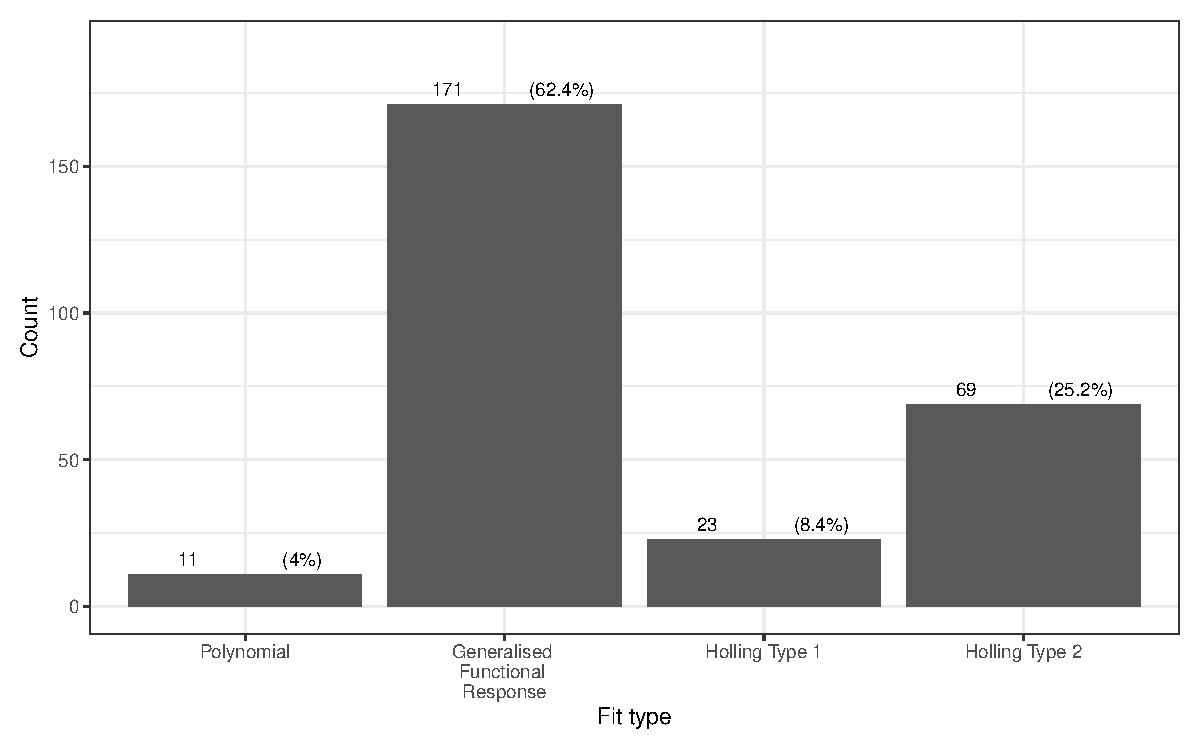
\includegraphics[width=1\textwidth]{../Results/Model_Comparison_Barchart.pdf}
	\caption{ID count by best fit model type}
\end{figure}

\subsection{Data subsets}

The dataset was preliminarily plotted in terms of eight factors: habitat, expermental conditions (lab/field/enclosure), consumer and rescoure thermal type, consumer and resource foraging movement and consumer and resource movement dimensionalty. All of these had a very similar ratio between the different best fits to that of the whole dataset, as can be seen from the four examples in Table 1. The few factors with slightly more varied proportions can be explained by the low quantity of data for that trait, for example passive resource foraging movement, which has only seven records. No particular trait was best fitted by a particular model, which is why the second focus of this paper is filter feeders. 

\begin{table}[ht!]
	\centering\csvreader[
	respect all,
	autotabular
	]{../Results/habitat_table.csv}{}{\csvlinetotablerow}
\end{table}

\begin{table}[ht!]
	\centering\csvreader[
	respect all,
	autotabular,
	]{../Results/labfield_table.csv}{}{\csvlinetotablerow}
\end{table}

\begin{table}[ht!]
	\centering\csvreader[
	respect all,
	autotabular
	]{../Results/res_movement_table.csv}{}{\csvlinetotablerow}
\end{table}

\begin{table}[ht!]
	\centering\csvreader[
	respect all,
	autotabular
	]{../Results/con_movement_table.csv}{}{\csvlinetotablerow}
	\caption{Different fit proportions in terms of various factors. The fit proportions shown by the overall data are shown at the bottom of each table.}
\end{table}

\subsection{Feeding mode}

Each of the IDs best fitted by a Holling type I response was allocated a feeding mode (either filter feeder or non-filter feeder), with the aim of exploring the 2004 claim by Jeschke et al.\parencite{Jeschke2004} that only filter feeders can display a Holling type I functional response. This allocation, along with the reference, can be seen in Table 2 and has been done according to the defintion of a filter feeder in the 2004 paper by Jeschke et al. This is a very broad definition that includes suspension feeders, trap builders, sediment filter feeders, those that only filter feed at certain stages in their lifecycle and also those that change feeding strategies according to prey abundance \parencite{Jeschke2004}.
From Table 2, it is apparent that a total of 11 of the 15 IDs best fit by a Holling type I functional response are classed as non-filter feeders.
This result is not insignifcant ($p < 2.2\times10^{-16}$ using G goodness of fit test). Figure 2 shows an example of a clearly linear functional response for a non-filter feeder consumer that is best fitted by the Holling type I equation.

\begin{table}[h!]
	\small
	\begin{tabular} {| l | l | l |}  \hline
		\textbf{ID} & \textbf{Taxa and Lifestage} & \textbf{Feeding Mode with Reference} \\ \hline
		695 & Stethorus punctum (Adult) & Non-Filter Feeder \parencite{Stethorus}  \\ \hline
		39839 & Rhyacophila dorsalis (Second Instar) &  Non-Filter Feeder \parencite{Rhyacophila}  \\ \hline
		39866 & Notonecta maculata (Fourth instar) & Non-Filter Feeder \parencite{Notonecta}  \\ \hline
		39890 & Anomalagrion hastatum  (Final Instar) &  Non-Filter Feeder \parencite{Anomalagrion}  \\ \hline
		39896, 39905 & Chaoborus americanus ( Fourth instar) & Non-Filter Feeder  \parencite{Chaoborus}  \\ \hline
		39920 & Ranatra dispar (Fifth instar)  &  Non-Filter Feeder \parencite{Ranatra}  \\ \hline
		40010 & Nereis (Hediste) diversicolor (Adult) & Filter Feeder \parencite{Nereis}  \\ \hline
		40019 & Parabroteas sarsi (Adult) & Filter Feeder \parencite{Copepod}  \\ \hline
		40026 &  Cyclops kolensis (Adult) & Non-Filter Feeder \parencite{Cyclops}  \\ \hline
		40066 & Praunus flexuosus (Adult) & Filter Feeder \parencite{Praunus}  \\ \hline
		40089, 40094, 40097 & Sander vitreus (Juvenile) &  Non-Filter Feeder \parencite{Sander}  \\ \hline
		400121 & Aurelia aurita (Juvenile) & Filter Feeder \parencite{Aurelia} \\ \hline
	\end{tabular}
	\caption{The consumers of functional responses best fit by a Holling Type I fit. Feeding mode has been based on the defintion used by Jeschke et al \parencite{Jeschke2004}}
\end{table}

\begin{figure}[ht!]
	\centering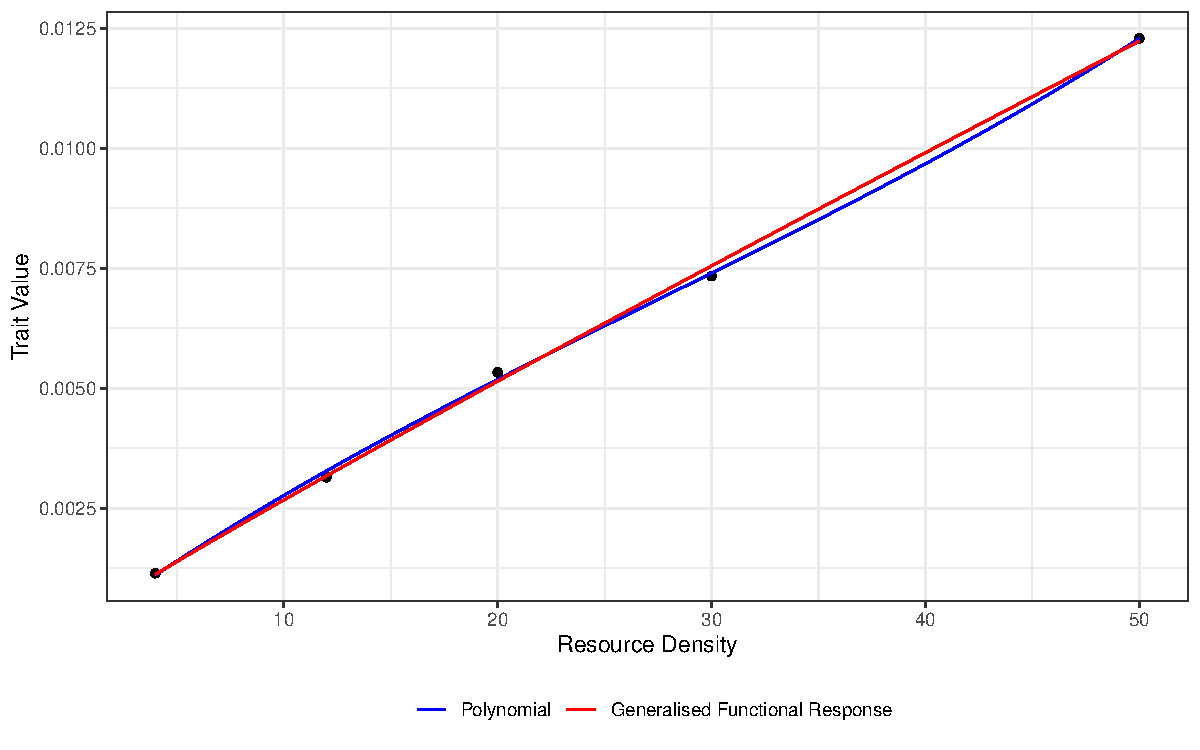
\includegraphics[width=1\textwidth]{../Results/Holling1_example.pdf}
	\caption{Functional response for a non-filter feeder consumer with Holling I best fit (ID = 39920, $q = -.0.055$, $h = 0$)}
\end{figure}


%%%%%%%%%%%%%%%% DISCUSSION %%%%%%%%%%%%%%%%


\section{Discussion}

\subsection{Mechanistic vs Phenomenological Models}

Functional response data are much better explained by the Holling mechanistic models than by a polynomial. This was to be expected, since the parameters in a polynomial do not correspond to biologically meaningful attributes and therefore have no underpinning scientific reasoning.
This is not to say that another mechanistic model might not describe the functional response with even more accuracy; however it does show the value of having models with a biological basis and provides evidence for their outperforming of phenomenological models.

\subsection{The Holling type I response}

The discrepancy between the expected and observed numbers of non-filter feeders with a type I functional response could be explained in two ways:

1) The limiting values of $a$ and $h$ used to subset the Holling type I response from the generalised functional response could have been inadequate, as they were not chosen using a mathematical method. As well as some functional responses being mis-classified as type I, some functional responses that should have been type I may have been missed.

2) Both Holling type II and III functional responses are linear away from the prey density limits. It is possible that not enough data were collected at very low and very high prey densities to display a type II or type III functional response, which is why they have been interpretted as type I.

Several different models have now been produced and  further work has been done to refine the Holling models, with modifications to account for both predator and prey size \parencite{Aljetlawi2004}, foraging dimensionality \parencite{Pawar2012} and changes over spatial scales \parencite{Rincon2017}, among others, all of which could impact the results of this study. The work by Seo and DeAngelis in describing the type I response shows a much more complicated dynamical system than formerly hypothesised \parencite{Seo2011}, which, if considered in this paper, could have provided evidence for the type I exclusivity to filter feeders. Many different models could further be applied to the empirical dataset to better understand the functional responses of both filter and non-filter feeders.

\subsection{The Holling type II and type III responses}

Although not an interest of this paper, it is worth noting the high proportion of IDs with a type III response as the best fit, given that type II is considered to be the most common generally \parencite{Holling1959b}. This is most likely explained by the strict boundaries imposed between the two types. The fitting and tests done in this paper do not reflect the complexities of the two types or the overlaps that are commonly seen. If the plots of those IDs classed as type III are viewed, it can be seen that many better resemble a type II curve ( an example ID is shown in figure 3), suggesting further differentiation is needed than just setting $q\approx0$. This could be because this work has not taken into account intermediate functional responses, which may better explain much of the dataset than the pure repsonses \parencite{Jeschke2004}.

\begin{figure}[ht!]
	\centering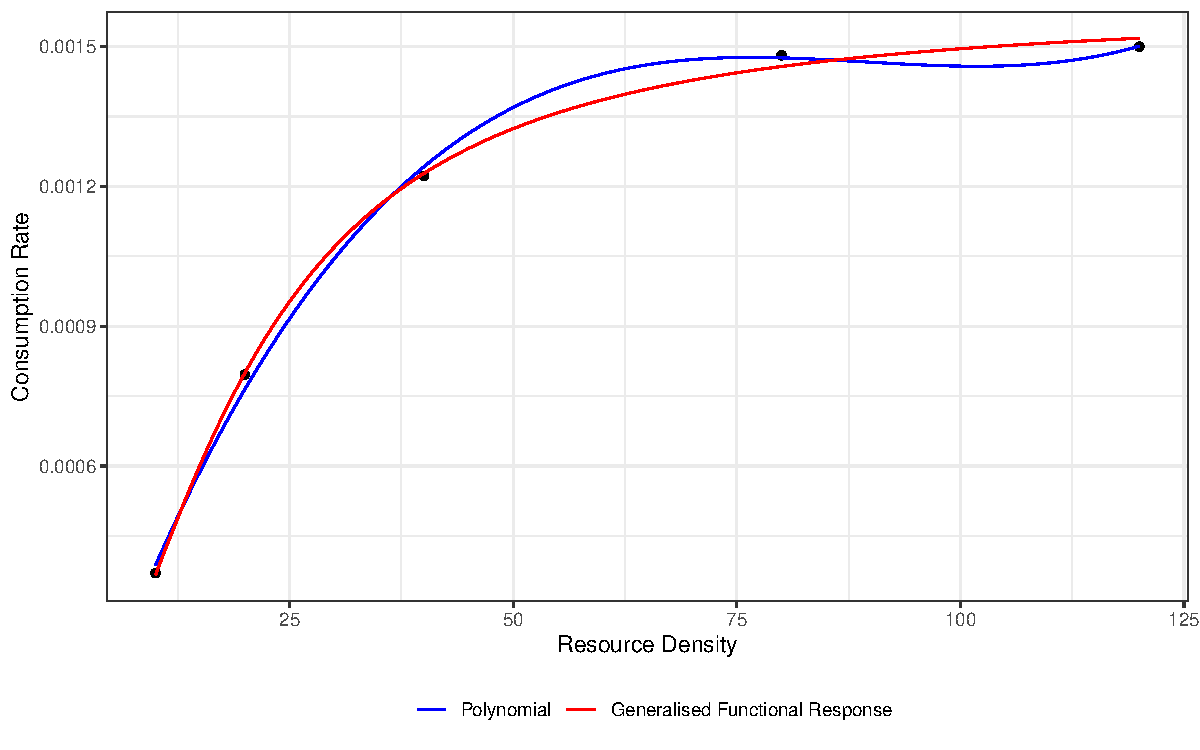
\includegraphics[width=1\textwidth]{../Results/GFR_Holling2_example.pdf}
	\caption{Holling Type II shape for a functional respnse best fit by a general functional response equation (ID = 39864, $q = 0.764$, $h = 632$)}
\end{figure}

\subsection{Concluding Remarks}

In the case of the Holling models and a polynomial, mechanistic models fit significantly better to an empirical dataset than phenomenological models. Although this might not be true for all mechanistic models as it depends on the accuracy of the model in describing nature, this is strong evidence for the superiority of mechanistic models over phenomenologial models.

Within the limits of the data provided, a Holling type I response is not exclusive to filter feeders, as has been previously suggested. However this may be due to a number of factors and so further research is required, perhaps using more sophisticated versions of Holling's models, to gain a more accurate picture.


\newpage
\printbibliography

\end{document}
}

\begin{document}

\begin{titlepage} % Suppresses headers and footers on the title page
	
	\centering % Centre everything on the title page
	
	\scshape % Use small caps for all text on the title page
	
	\vspace*{\baselineskip} % White space at the top of the page
	
	%------------------------------------------------
	
	%	Title
	
	%------------------------------------------------
	
	\rule{\textwidth}{1.6pt}\vspace*{-\baselineskip}\vspace*{2pt} % Thick horizontal rule
	
	\rule{\textwidth}{0.4pt} % Thin horizontal rule
	
	\vspace{0.75\baselineskip} % Whitespace above the title
	
	{\LARGE A comparison of a phenomenological model with Holling's mechanistic models for functional responses, focusing on filter and non-filter consumer feeding modes\\} % Title
	
	\vspace{0.75\baselineskip} % Whitespace below the title
	
	\rule{\textwidth}{0.4pt}\vspace*{-\baselineskip}\vspace{3.2pt} % Thin horizontal rule
	
	\rule{\textwidth}{1.6pt} % Thick horizontal rule
	
	\vspace{2\baselineskip} % Whitespace after the title block
	
	%------------------------------------------------
	
	%	Subtitle
	
	%------------------------------------------------
	
	Computational Methods in Ecology and Evolution MRes
	\vspace{0.5\baselineskip}
	
	 MiniProject % Subtitle or further description
	
	\vspace*{3\baselineskip} % Whitespace under the subtitle
	
	%------------------------------------------------
	
	%	Editor(s)
	
	%------------------------------------------------
	
	\vspace{0.5\baselineskip} % Whitespace before the editors
	
	{\scshape\Large Lucy Goodyear\\
		Department of life Sceinces \\
		Imperial College London\\} % Editor list
	
	\textit{lucy.goodyear19@imperial.ac.uk}
	\date{}
	
	\vspace*{3\baselineskip} % Whitespace under the subtitle
	
	Word Count: \wordcount
	
\end{titlepage}
	
\section*{Abstract}
Functional responses, the relationship between a consumption rate and resource density, can be categorised into three types. The first, the type I response, is a linear relationship, exhibited by some filter feeders. The second, the type II response, also known as the Holling Model or the basic functional response, is the most common and represents a response with a non-zero handling time. The third, the type III response, is the generalised functional response, from which the other two can be produced, and is linked to predator switching and learning. All three are examples of a mechanistic model, which is a model based on biological principles. In this paper, the type III response (the generalised functional response), and by extension the other two types, are compared against a phenomenological model, a polynomial, and shown to be a significantly better fit to empirical data. This provides evidence for the outperformance of mechanistic models over phenomenological models. 

Those datasets that were fitted best by the generalised functional response were then subsetted into the three different functional response types in order to identify those best fitted by the Holling type I model. By reviewing these datasets in terms of feeding mode, the claim by Jeschke et al. in their 2004 paper that "type I functional responses are exclusive to filter feeders" is tested and contradicting data is found. This does not conclusively reject the claim, as there are many other factors that could have influenced this result, but rather suggests further study should be done in this area.

\newpage

\linenumbers


%%%%%%%%%%%%%%%% INTRODUCTION %%%%%%%%%%%%%%%%


\section{Introduction}
The term functional response refers to the relationship between a consumer's consumption rate and the density of its prey \parencite{Solomon1949}.  The first mechanistic mathematical approach to functional responses was conducted by Holling in 1959 \parencite{Holling1959b}. Holling constructed an artificial functional response experiment and discovered that the consumption rate is related to prey in terms of two constants: instantaneous rate of discovery and handling time. The instantaneous rate of discovery corresponds to the likelihood of a predator finding an individual prey, expressed as the volume or area searched per unit of time.
The handling time is any time not spent in actively searching for prey. There have been discussions on the different physical activities that handling time includes, such as digestion, time spent consuming prey, time spent hunting prey etc. \parencite{Jeschke2002, Holling1966} but for the purposes of this paper, we are assuming handling time is time spent on any non-foraging activities.
This functional response is the most common in nature and is known as the basic functional response \parencite{Holling1959b}.

In an earlier paper of the same year, Holling describes the shapes of the three functional responses \parencite{Holling1959a} where his experimentally dervied basic functional response can be seen to describe a type II functional response.

Other attempts at modelling functional responses have been made using different assumptions and mathematics; these are discussed by Holling in a later paper, in which he remarks on the lack of biological context in most of the other options \parencite{Holling1965}. Since then, further models have been formalised and changes made to the original Holling equations but these were not used in this paper's hypothesis and  will only be considered in the discussion. 

\bigskip

The type III functional response was modelled using computer simulations and labelled as the generalised functional response by Holling in a later paper \parencite{Holling1965}, with types I and II being limiting conditions. However, type III was not described mathematically until 1977 by Real, who derived it using Holling's type II functional response equation and first-order kinetic interactions \parencite{Real1977}.
 
The generalised functional response equation is written below, where $c$ is the consumer consumption rate, $a$ is the instantaneous rate of discovery, $x$ is the resource density, $h$ is the handling time and $q$ is a variable with as yet unknown biological meaning. It has been hypothesised that $q$ could be related to predator learning and is `the number of encounters...a predator must have with a prey item before becoming maximally efficient at utilizing the prey item as a resource' \parencite{Real1977}.

\begin{equation}
c = \frac{ax_R^{q + 1}}{1 + hax_R^{q + 1}}
\end{equation}

\bigskip

It can be shown that the type II functional response is a special case of the generalised functional response by setting $q = 0$. In terms of Real's interpretation of $q$, this means that the predator `is always maximally efficient on the prey item'  \parencite{Real1977} in a type II response.

\begin{equation}
c = \frac{ax_R}{1 + hax_R}
\end{equation}

\bigskip

 In type I, the handling time is negligible, reducing the second term in the denominator to almost zero, leaving us with a linear relationship:

\begin{equation}
c = ax_R
\end{equation}

Type I responses are to be found in filter feeders, where the predation rate is directly  proportional to the prey density \parencite{Jeschke2004}. This is because filter feeders are able to do activities simultaneously so can effectively spend all their time foraging. There is normally a hard cut-off at very high prey densities, indicating a maximum number of prey that can be caught. \parencite{Jeschke2004}. 

This paper aims to look at whether the generalised functional response equation (a mechanistic model) or a polynomial (a phenomenological model) fits best to empirical functional response data. The polynomial has no biological meaning, so the comparison is effectively one of phenomenological vs mechanistic models. The null hypothesis is that the mechanistic model is no better than a phenomenological model and so the data will be best fit by each model roughly half the time.

By fitting both the general functional response model and a polynomial to 295 empirical datasets, the proportion of best fits by model can be compared. The functional response types were also compared by subsetting by the limiting conditions of type I and type II functional responses, i.e. filtering by the values of $h$ and $q$ respectively, gaining information on the split between the three types. The data can then be subsetted by different metadata fields, such as habitat, in order to look for model fitting trends.

The second part of this paper focusses on the functional response of  filter feeders. In previous work, it has been shown that, although the majority of filter feeders do not show a type I response, the type I reponse is only possible for filter feeders \parencite{Jeschke2004}.  Type I functional responses are characterised by two main conditions: handling time must be negligible and the consumer must always spend the maximal time and effort foraging, the only exception being once the gut is full (satiation condition) \parencite{Jeschke2002}. Many filter feeders have a negligible handing time because they are able to catch prey at the same time as performing other activities, resulting in effectively all of their time being spent foraging. Some filter feeders also adhere to the satiation condition but not many. Both conditions must be met in order for the functional response to be type I, but both conditions could also be met when the resulting functional response is of a different type. This is why it is claimed that the majority of filter feeders (and all non-filter feeders) do not show a type 1 response \parencite{Jeschke2004, Deville2013, Porter1983}. Here, the exclusivity of a type I response to filter feeders is explored in terms of Real's definition of $q$ and derivation of the type III functional response, looking at functional responses when $q$ is not confined to any limits \parencite{Real1977}.  It is expected that there will be full adherence to the paper of Jeschke et al. and so no Holling type I responses are expected to best fit any non-filter feeders.


%%%%%%%%%%%%%%%%%% METHODS %%%%%%%%%%%%%%%%%%%


\section{Methods}

\subsection{Data}

The dataset used is a collection of 4507 records, grouped into 308 IDs, each of which corresponds to a different functional response. The data have been collected from various lab and field experiments, conducted globally, and measure the rate of consumption of a single resource by a consumer, along with various metadata, such as habitat and taxa. There are 68 fields but only 11 have been considered in this paper: ID, consumption rate and resource denisity for fitting the models; consumer foraging movement, resource foraging movement, habitat, experimental conditions (lab/field/enclosure), resource movement dimensionality, consumer movement dimensionality, resource thermal type and consumer thermal type for subsetting the data and looking for trends.

\subsection{Computing Tools}

\subsubsection{Data preparation—R}

Data was prepared for fitting using R v.3.6.1 \parencite{R} because of the ease of viewing data and of accessing and manipulating dataframes. First, the data is subsetted by the necessary columns, all records with missing consumption rates and all IDs with fewer than 5 records are removed (to reduce the possibility of overfitting), which leaves 295 IDs remaining. The data preparation script then generates initial starting values for $a$ and $h$ for the general functional response fit. A new dataframe, including subsetted data and initial starting values for $a$ and $h$, is saved to a csv file.

\subsubsection{Model Fitting — Python}
The starting value optimisation and fitting script is done using Python v.3.7.4 \parencite{Python}. For the polynomial fit, there is an in-built Python function, which also calculates starting values and fit statistics. For the general functional response fit, a Gaussian sample of 6 (chosen for speed of programme execution) is generated around the estimated starting values and each combinatiom of these sample values is used to fit a model to the dataset, resulting in 36 different fits. The AIC, BIC and residual sums of squares (RSS) are calculated for each ID and the starting values for the model with the lowest AIC are chosen as the best fit \parencite{Johnson2004}.  These calculations are perfomed for each ID using parallelisation and the best fit parameters and statsitics are stored in a new dataframe and then saved as a csv for importing into R for the plotting and analysis script.

Functions are saved in a separate Python script and have been generalised to allow importing into future programmes. Two inbuilt Python packages have been used: itertools to try all combinations of the start values, and multiprocessing to allow parallelisation \parencite{Python}. The packages lmfit \parencite{lmfit} v.0.9.14, NumPy \parencite{NumPy} v.1.18.1 and pandas \parencite{pandas} v.0.24.2 were used. NumPy contains the polynomial fitting function as well as different mathematical values, such as $\pi$. The package lmfit allows the use of parameters when fitting a model and pandas is a dataframe tool.

\subsubsection{Plotting and Analysis — R}
The plotting and analysis script has been written in R due to the ease of graphical representation in RStudio and statistical functionality. Four packages are used: ggplot2 \parencite{ggplot2} for visualisation; tidyverse \parencite{tidyverse} for easy data manipulation; DescTools {\parencite{DescTools}}  for stastical tests; and janitor \parencite{janitor} to create flexible tables. After reviewing the datasets, those IDs which haven't been fitted properly are discarded. Some of the inaccurately fitted datasets have a large number of points at very low x-values and then a few at very high x-values, a logarithmic transformation could have been performed on these prior to fitting, but this option was discarded in favour of maintaining the biological significance of $a$ and $h$. This left 280 IDs remaining for analysis.

The script compares RSS, AIC and BIC for each model within each ID and chooses the best fit model based on at least two out of three agreements between these statstics. RSS is used as-is instead of calculating $R^{2}$ due to the new numerous pitfalls in calculating this statistic for non-linear regressions \parencite{kvalseth1985}.
AIC and BIC were chosen because they are the currently viewed as the most appropriate best-fit statsitics \parencite{Johnson2004}. The spread of best fits was compared graphically and a measure of the significance of the resulting proportion of fits between the phenomenological and the mechanistic model was obtained by performing both a G-test of goodness-of-fit and a chi-square goodness-of-fit test. 

The data is then subsetted into the three Holling types by setting any ID with the generalised fucntional response as best fit and $-0.3<q<0.3$ as Holling type II, and any Holling type II with $h<0.1$ as Holling type I. Given $q$ is given no limits in the fitting script, $0.3$ was chosen as the limiting boundary for $q$ visually, based on the whether the resulting plots exhibited a Holling type II or Holling type I shape.
Plots and tables of eight different metadata fields and a table showing the proportion of best fit models in terms of feeding mode are then generated and a G-test of goodness-of-fit is performed to test the significance of the proportion of non-filter feeders best fitted by a Holling type I response.

\subsubsection{Run Script — Bash}

Bash was chosen to join the above scripts into a clear, reproducible workflow because it can run R and Python scripts simply and easily, as well as compile latex files with references.


%%%%%%%%%%%%%%%%% RESULTS %%%%%%%%%%%%%%%%%%%


\section{Results}

\subsection{Mechanistic vs Phenomenological Models}

The findings of a comparison between the mechanistic model and the phenomenological models are shown in Figure 1. It is clear that the mechanistic models are a much better fit. 95.4\% of the data was best fitted by the mechanstic model, which accounts for 267 of 280 IDs. This is highly significtant ($p < 2.2\times10^{-16}$ for both G-test of goodness-of-fit and chi-square goodness-of-fit test), showing that the Holling mechanstic models fit empirical data much better than a polynomial.

\begin{figure}[ht!]
	\centering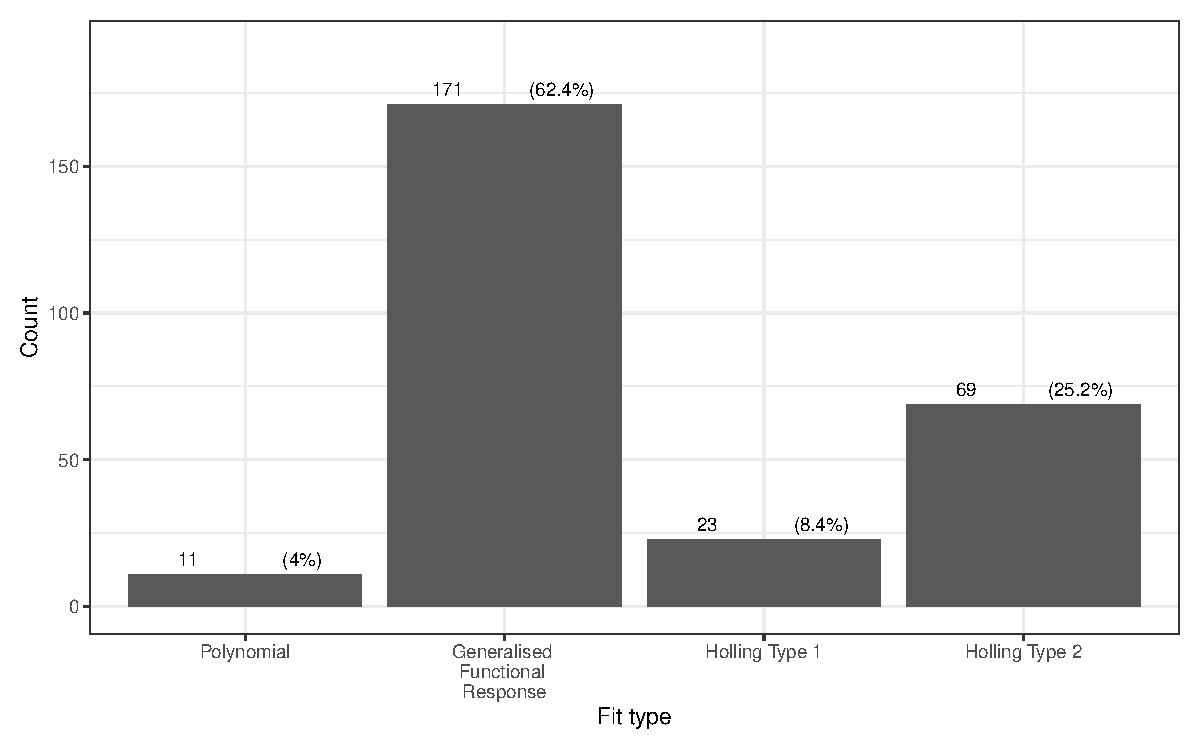
\includegraphics[width=1\textwidth]{../Results/Model_Comparison_Barchart.pdf}
	\caption{ID count by best fit model type}
\end{figure}

\subsection{Data subsets}

The dataset was preliminarily plotted in terms of eight factors: habitat, expermental conditions (lab/field/enclosure), consumer and rescoure thermal type, consumer and resource foraging movement and consumer and resource movement dimensionalty. All of these had a very similar ratio between the different best fits to that of the whole dataset, as can be seen from the four examples in Table 1. The few factors with slightly more varied proportions can be explained by the low quantity of data for that trait, for example passive resource foraging movement, which has only seven records. No particular trait was best fitted by a particular model, which is why the second focus of this paper is filter feeders. 

\begin{table}[ht!]
	\centering\csvreader[
	respect all,
	autotabular
	]{../Results/habitat_table.csv}{}{\csvlinetotablerow}
\end{table}

\begin{table}[ht!]
	\centering\csvreader[
	respect all,
	autotabular,
	]{../Results/labfield_table.csv}{}{\csvlinetotablerow}
\end{table}

\begin{table}[ht!]
	\centering\csvreader[
	respect all,
	autotabular
	]{../Results/res_movement_table.csv}{}{\csvlinetotablerow}
\end{table}

\begin{table}[ht!]
	\centering\csvreader[
	respect all,
	autotabular
	]{../Results/con_movement_table.csv}{}{\csvlinetotablerow}
	\caption{Different fit proportions in terms of various factors. The fit proportions shown by the overall data are shown at the bottom of each table.}
\end{table}

\subsection{Feeding mode}

Each of the IDs best fitted by a Holling type I response was allocated a feeding mode (either filter feeder or non-filter feeder), with the aim of exploring the 2004 claim by Jeschke et al.\parencite{Jeschke2004} that only filter feeders can display a Holling type I functional response. This allocation, along with the reference, can be seen in Table 2 and has been done according to the defintion of a filter feeder in the 2004 paper by Jeschke et al. This is a very broad definition that includes suspension feeders, trap builders, sediment filter feeders, those that only filter feed at certain stages in their lifecycle and also those that change feeding strategies according to prey abundance \parencite{Jeschke2004}.
From Table 2, it is apparent that a total of 11 of the 15 IDs best fit by a Holling type I functional response are classed as non-filter feeders.
This result is not insignifcant ($p < 2.2\times10^{-16}$ using G goodness of fit test). Figure 2 shows an example of a clearly linear functional response for a non-filter feeder consumer that is best fitted by the Holling type I equation.

\begin{table}[h!]
	\small
	\begin{tabular} {| l | l | l |}  \hline
		\textbf{ID} & \textbf{Taxa and Lifestage} & \textbf{Feeding Mode with Reference} \\ \hline
		695 & Stethorus punctum (Adult) & Non-Filter Feeder \parencite{Stethorus}  \\ \hline
		39839 & Rhyacophila dorsalis (Second Instar) &  Non-Filter Feeder \parencite{Rhyacophila}  \\ \hline
		39866 & Notonecta maculata (Fourth instar) & Non-Filter Feeder \parencite{Notonecta}  \\ \hline
		39890 & Anomalagrion hastatum  (Final Instar) &  Non-Filter Feeder \parencite{Anomalagrion}  \\ \hline
		39896, 39905 & Chaoborus americanus ( Fourth instar) & Non-Filter Feeder  \parencite{Chaoborus}  \\ \hline
		39920 & Ranatra dispar (Fifth instar)  &  Non-Filter Feeder \parencite{Ranatra}  \\ \hline
		40010 & Nereis (Hediste) diversicolor (Adult) & Filter Feeder \parencite{Nereis}  \\ \hline
		40019 & Parabroteas sarsi (Adult) & Filter Feeder \parencite{Copepod}  \\ \hline
		40026 &  Cyclops kolensis (Adult) & Non-Filter Feeder \parencite{Cyclops}  \\ \hline
		40066 & Praunus flexuosus (Adult) & Filter Feeder \parencite{Praunus}  \\ \hline
		40089, 40094, 40097 & Sander vitreus (Juvenile) &  Non-Filter Feeder \parencite{Sander}  \\ \hline
		400121 & Aurelia aurita (Juvenile) & Filter Feeder \parencite{Aurelia} \\ \hline
	\end{tabular}
	\caption{The consumers of functional responses best fit by a Holling Type I fit. Feeding mode has been based on the defintion used by Jeschke et al \parencite{Jeschke2004}}
\end{table}

\begin{figure}[ht!]
	\centering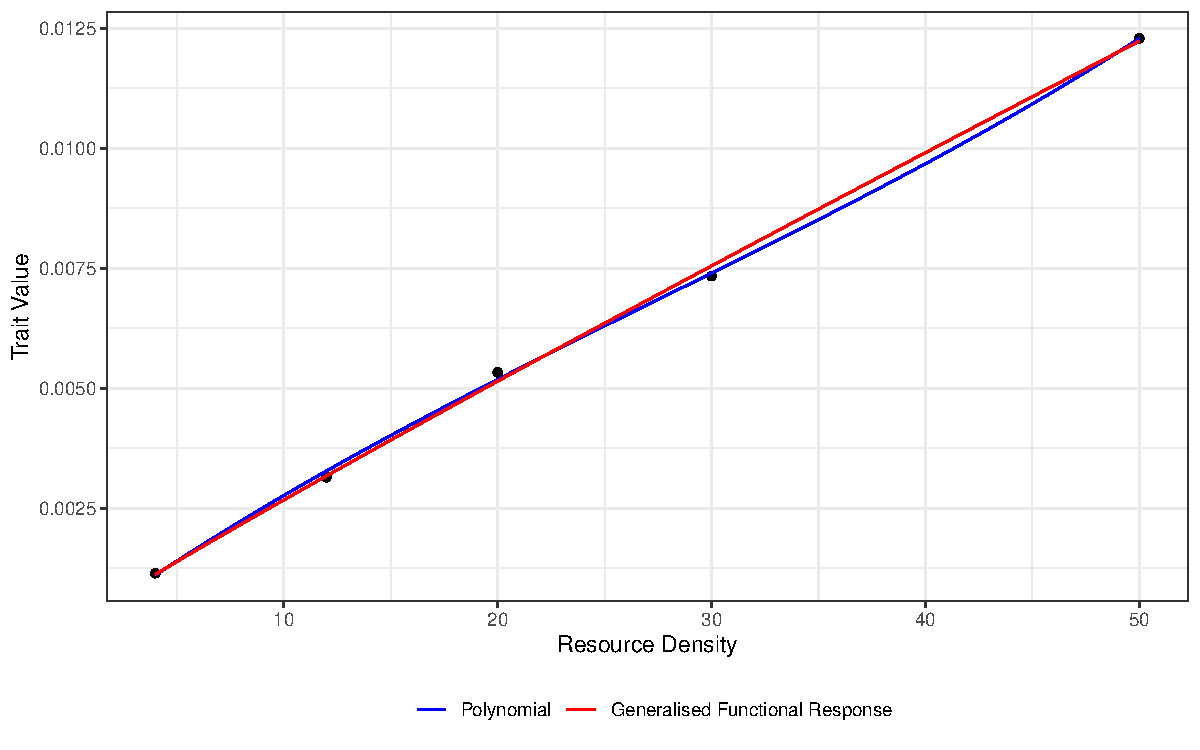
\includegraphics[width=1\textwidth]{../Results/Holling1_example.pdf}
	\caption{Functional response for a non-filter feeder consumer with Holling I best fit (ID = 39920, $q = -.0.055$, $h = 0$)}
\end{figure}


%%%%%%%%%%%%%%%% DISCUSSION %%%%%%%%%%%%%%%%


\section{Discussion}

\subsection{Mechanistic vs Phenomenological Models}

Functional response data are much better explained by the Holling mechanistic models than by a polynomial. This was to be expected, since the parameters in a polynomial do not correspond to biologically meaningful attributes and therefore have no underpinning scientific reasoning.
This is not to say that another mechanistic model might not describe the functional response with even more accuracy; however it does show the value of having models with a biological basis and provides evidence for their outperforming of phenomenological models.

\subsection{The Holling type I response}

The discrepancy between the expected and observed numbers of non-filter feeders with a type I functional response could be explained in two ways:

1) The limiting values of $a$ and $h$ used to subset the Holling type I response from the generalised functional response could have been inadequate, as they were not chosen using a mathematical method. As well as some functional responses being mis-classified as type I, some functional responses that should have been type I may have been missed.

2) Both Holling type II and III functional responses are linear away from the prey density limits. It is possible that not enough data were collected at very low and very high prey densities to display a type II or type III functional response, which is why they have been interpretted as type I.

Several different models have now been produced and  further work has been done to refine the Holling models, with modifications to account for both predator and prey size \parencite{Aljetlawi2004}, foraging dimensionality \parencite{Pawar2012} and changes over spatial scales \parencite{Rincon2017}, among others, all of which could impact the results of this study. The work by Seo and DeAngelis in describing the type I response shows a much more complicated dynamical system than formerly hypothesised \parencite{Seo2011}, which, if considered in this paper, could have provided evidence for the type I exclusivity to filter feeders. Many different models could further be applied to the empirical dataset to better understand the functional responses of both filter and non-filter feeders.

\subsection{The Holling type II and type III responses}

Although not an interest of this paper, it is worth noting the high proportion of IDs with a type III response as the best fit, given that type II is considered to be the most common generally \parencite{Holling1959b}. This is most likely explained by the strict boundaries imposed between the two types. The fitting and tests done in this paper do not reflect the complexities of the two types or the overlaps that are commonly seen. If the plots of those IDs classed as type III are viewed, it can be seen that many better resemble a type II curve ( an example ID is shown in figure 3), suggesting further differentiation is needed than just setting $q\approx0$. This could be because this work has not taken into account intermediate functional responses, which may better explain much of the dataset than the pure repsonses \parencite{Jeschke2004}.

\begin{figure}[ht!]
	\centering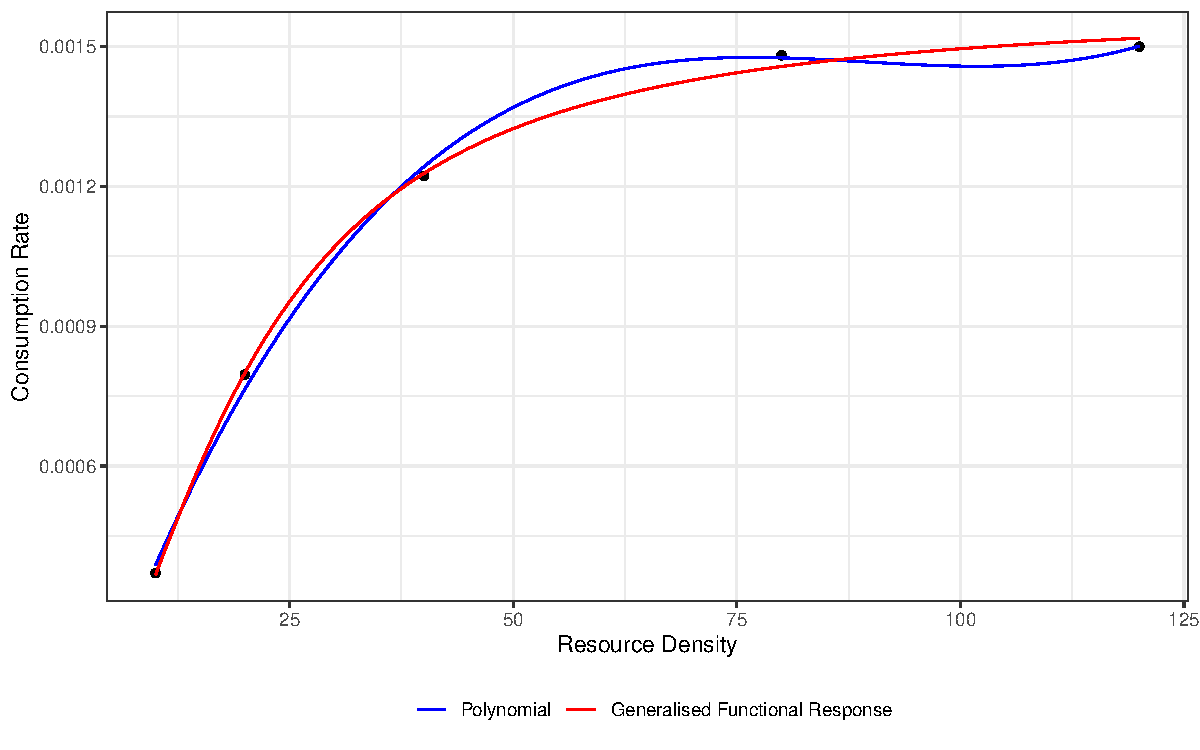
\includegraphics[width=1\textwidth]{../Results/GFR_Holling2_example.pdf}
	\caption{Holling Type II shape for a functional respnse best fit by a general functional response equation (ID = 39864, $q = 0.764$, $h = 632$)}
\end{figure}

\subsection{Concluding Remarks}

In the case of the Holling models and a polynomial, mechanistic models fit significantly better to an empirical dataset than phenomenological models. Although this might not be true for all mechanistic models as it depends on the accuracy of the model in describing nature, this is strong evidence for the superiority of mechanistic models over phenomenologial models.

Within the limits of the data provided, a Holling type I response is not exclusive to filter feeders, as has been previously suggested. However this may be due to a number of factors and so further research is required, perhaps using more sophisticated versions of Holling's models, to gain a more accurate picture.


\newpage
\printbibliography

\end{document}
}

\begin{document}

\begin{titlepage} % Suppresses headers and footers on the title page
	
	\centering % Centre everything on the title page
	
	\scshape % Use small caps for all text on the title page
	
	\vspace*{\baselineskip} % White space at the top of the page
	
	%------------------------------------------------
	
	%	Title
	
	%------------------------------------------------
	
	\rule{\textwidth}{1.6pt}\vspace*{-\baselineskip}\vspace*{2pt} % Thick horizontal rule
	
	\rule{\textwidth}{0.4pt} % Thin horizontal rule
	
	\vspace{0.75\baselineskip} % Whitespace above the title
	
	{\LARGE A comparison of a phenomenological model with Holling's mechanistic models for functional responses, focusing on filter and non-filter consumer feeding modes\\} % Title
	
	\vspace{0.75\baselineskip} % Whitespace below the title
	
	\rule{\textwidth}{0.4pt}\vspace*{-\baselineskip}\vspace{3.2pt} % Thin horizontal rule
	
	\rule{\textwidth}{1.6pt} % Thick horizontal rule
	
	\vspace{2\baselineskip} % Whitespace after the title block
	
	%------------------------------------------------
	
	%	Subtitle
	
	%------------------------------------------------
	
	Computational Methods in Ecology and Evolution MRes
	\vspace{0.5\baselineskip}
	
	 MiniProject % Subtitle or further description
	
	\vspace*{3\baselineskip} % Whitespace under the subtitle
	
	%------------------------------------------------
	
	%	Editor(s)
	
	%------------------------------------------------
	
	\vspace{0.5\baselineskip} % Whitespace before the editors
	
	{\scshape\Large Lucy Goodyear\\
		Department of life Sceinces \\
		Imperial College London\\} % Editor list
	
	\textit{lucy.goodyear19@imperial.ac.uk}
	\date{}
	
	\vspace*{3\baselineskip} % Whitespace under the subtitle
	
	Word Count: \wordcount
	
\end{titlepage}
	
\section*{Abstract}
Functional responses, the relationship between a consumption rate and resource density, can be categorised into three types. The first, the type I response, is a linear relationship, exhibited by some filter feeders. The second, the type II response, also known as the Holling Model or the basic functional response, is the most common and represents a response with a non-zero handling time. The third, the type III response, is the generalised functional response, from which the other two can be produced, and is linked to predator switching and learning. All three are examples of a mechanistic model, which is a model based on biological principles. In this paper, the type III response (the generalised functional response), and by extension the other two types, are compared against a phenomenological model, a polynomial, and shown to be a significantly better fit to empirical data. This provides evidence for the outperformance of mechanistic models over phenomenological models. 

Those datasets that were fitted best by the generalised functional response were then subsetted into the three different functional response types in order to identify those best fitted by the Holling type I model. By reviewing these datasets in terms of feeding mode, the claim by Jeschke et al. in their 2004 paper that "type I functional responses are exclusive to filter feeders" is tested and contradicting data is found. This does not conclusively reject the claim, as there are many other factors that could have influenced this result, but rather suggests further study should be done in this area.

\newpage

\linenumbers


%%%%%%%%%%%%%%%% INTRODUCTION %%%%%%%%%%%%%%%%


\section{Introduction}
The term functional response refers to the relationship between a consumer's consumption rate and the density of its prey \parencite{Solomon1949}.  The first mechanistic mathematical approach to functional responses was conducted by Holling in 1959 \parencite{Holling1959b}. Holling constructed an artificial functional response experiment and discovered that the consumption rate is related to prey in terms of two constants: instantaneous rate of discovery and handling time. The instantaneous rate of discovery corresponds to the likelihood of a predator finding an individual prey, expressed as the volume or area searched per unit of time.
The handling time is any time not spent in actively searching for prey. There have been discussions on the different physical activities that handling time includes, such as digestion, time spent consuming prey, time spent hunting prey etc. \parencite{Jeschke2002, Holling1966} but for the purposes of this paper, we are assuming handling time is time spent on any non-foraging activities.
This functional response is the most common in nature and is known as the basic functional response \parencite{Holling1959b}.

In an earlier paper of the same year, Holling describes the shapes of the three functional responses \parencite{Holling1959a} where his experimentally dervied basic functional response can be seen to describe a type II functional response.

Other attempts at modelling functional responses have been made using different assumptions and mathematics; these are discussed by Holling in a later paper, in which he remarks on the lack of biological context in most of the other options \parencite{Holling1965}. Since then, further models have been formalised and changes made to the original Holling equations but these were not used in this paper's hypothesis and  will only be considered in the discussion. 

\bigskip

The type III functional response was modelled using computer simulations and labelled as the generalised functional response by Holling in a later paper \parencite{Holling1965}, with types I and II being limiting conditions. However, type III was not described mathematically until 1977 by Real, who derived it using Holling's type II functional response equation and first-order kinetic interactions \parencite{Real1977}.
 
The generalised functional response equation is written below, where $c$ is the consumer consumption rate, $a$ is the instantaneous rate of discovery, $x$ is the resource density, $h$ is the handling time and $q$ is a variable with as yet unknown biological meaning. It has been hypothesised that $q$ could be related to predator learning and is `the number of encounters...a predator must have with a prey item before becoming maximally efficient at utilizing the prey item as a resource' \parencite{Real1977}.

\begin{equation}
c = \frac{ax_R^{q + 1}}{1 + hax_R^{q + 1}}
\end{equation}

\bigskip

It can be shown that the type II functional response is a special case of the generalised functional response by setting $q = 0$. In terms of Real's interpretation of $q$, this means that the predator `is always maximally efficient on the prey item'  \parencite{Real1977} in a type II response.

\begin{equation}
c = \frac{ax_R}{1 + hax_R}
\end{equation}

\bigskip

 In type I, the handling time is negligible, reducing the second term in the denominator to almost zero, leaving us with a linear relationship:

\begin{equation}
c = ax_R
\end{equation}

Type I responses are to be found in filter feeders, where the predation rate is directly  proportional to the prey density \parencite{Jeschke2004}. This is because filter feeders are able to do activities simultaneously so can effectively spend all their time foraging. There is normally a hard cut-off at very high prey densities, indicating a maximum number of prey that can be caught. \parencite{Jeschke2004}. 

This paper aims to look at whether the generalised functional response equation (a mechanistic model) or a polynomial (a phenomenological model) fits best to empirical functional response data. The polynomial has no biological meaning, so the comparison is effectively one of phenomenological vs mechanistic models. The null hypothesis is that the mechanistic model is no better than a phenomenological model and so the data will be best fit by each model roughly half the time.

By fitting both the general functional response model and a polynomial to 295 empirical datasets, the proportion of best fits by model can be compared. The functional response types were also compared by subsetting by the limiting conditions of type I and type II functional responses, i.e. filtering by the values of $h$ and $q$ respectively, gaining information on the split between the three types. The data can then be subsetted by different metadata fields, such as habitat, in order to look for model fitting trends.

The second part of this paper focusses on the functional response of  filter feeders. In previous work, it has been shown that, although the majority of filter feeders do not show a type I response, the type I reponse is only possible for filter feeders \parencite{Jeschke2004}.  Type I functional responses are characterised by two main conditions: handling time must be negligible and the consumer must always spend the maximal time and effort foraging, the only exception being once the gut is full (satiation condition) \parencite{Jeschke2002}. Many filter feeders have a negligible handing time because they are able to catch prey at the same time as performing other activities, resulting in effectively all of their time being spent foraging. Some filter feeders also adhere to the satiation condition but not many. Both conditions must be met in order for the functional response to be type I, but both conditions could also be met when the resulting functional response is of a different type. This is why it is claimed that the majority of filter feeders (and all non-filter feeders) do not show a type 1 response \parencite{Jeschke2004, Deville2013, Porter1983}. Here, the exclusivity of a type I response to filter feeders is explored in terms of Real's definition of $q$ and derivation of the type III functional response, looking at functional responses when $q$ is not confined to any limits \parencite{Real1977}.  It is expected that there will be full adherence to the paper of Jeschke et al. and so no Holling type I responses are expected to best fit any non-filter feeders.


%%%%%%%%%%%%%%%%%% METHODS %%%%%%%%%%%%%%%%%%%


\section{Methods}

\subsection{Data}

The dataset used is a collection of 4507 records, grouped into 308 IDs, each of which corresponds to a different functional response. The data have been collected from various lab and field experiments, conducted globally, and measure the rate of consumption of a single resource by a consumer, along with various metadata, such as habitat and taxa. There are 68 fields but only 11 have been considered in this paper: ID, consumption rate and resource denisity for fitting the models; consumer foraging movement, resource foraging movement, habitat, experimental conditions (lab/field/enclosure), resource movement dimensionality, consumer movement dimensionality, resource thermal type and consumer thermal type for subsetting the data and looking for trends.

\subsection{Computing Tools}

\subsubsection{Data preparation—R}

Data was prepared for fitting using R v.3.6.1 \parencite{R} because of the ease of viewing data and of accessing and manipulating dataframes. First, the data is subsetted by the necessary columns, all records with missing consumption rates and all IDs with fewer than 5 records are removed (to reduce the possibility of overfitting), which leaves 295 IDs remaining. The data preparation script then generates initial starting values for $a$ and $h$ for the general functional response fit. A new dataframe, including subsetted data and initial starting values for $a$ and $h$, is saved to a csv file.

\subsubsection{Model Fitting — Python}
The starting value optimisation and fitting script is done using Python v.3.7.4 \parencite{Python}. For the polynomial fit, there is an in-built Python function, which also calculates starting values and fit statistics. For the general functional response fit, a Gaussian sample of 6 (chosen for speed of programme execution) is generated around the estimated starting values and each combinatiom of these sample values is used to fit a model to the dataset, resulting in 36 different fits. The AIC, BIC and residual sums of squares (RSS) are calculated for each ID and the starting values for the model with the lowest AIC are chosen as the best fit \parencite{Johnson2004}.  These calculations are perfomed for each ID using parallelisation and the best fit parameters and statsitics are stored in a new dataframe and then saved as a csv for importing into R for the plotting and analysis script.

Functions are saved in a separate Python script and have been generalised to allow importing into future programmes. Two inbuilt Python packages have been used: itertools to try all combinations of the start values, and multiprocessing to allow parallelisation \parencite{Python}. The packages lmfit \parencite{lmfit} v.0.9.14, NumPy \parencite{NumPy} v.1.18.1 and pandas \parencite{pandas} v.0.24.2 were used. NumPy contains the polynomial fitting function as well as different mathematical values, such as $\pi$. The package lmfit allows the use of parameters when fitting a model and pandas is a dataframe tool.

\subsubsection{Plotting and Analysis — R}
The plotting and analysis script has been written in R due to the ease of graphical representation in RStudio and statistical functionality. Four packages are used: ggplot2 \parencite{ggplot2} for visualisation; tidyverse \parencite{tidyverse} for easy data manipulation; DescTools {\parencite{DescTools}}  for stastical tests; and janitor \parencite{janitor} to create flexible tables. After reviewing the datasets, those IDs which haven't been fitted properly are discarded. Some of the inaccurately fitted datasets have a large number of points at very low x-values and then a few at very high x-values, a logarithmic transformation could have been performed on these prior to fitting, but this option was discarded in favour of maintaining the biological significance of $a$ and $h$. This left 280 IDs remaining for analysis.

The script compares RSS, AIC and BIC for each model within each ID and chooses the best fit model based on at least two out of three agreements between these statstics. RSS is used as-is instead of calculating $R^{2}$ due to the new numerous pitfalls in calculating this statistic for non-linear regressions \parencite{kvalseth1985}.
AIC and BIC were chosen because they are the currently viewed as the most appropriate best-fit statsitics \parencite{Johnson2004}. The spread of best fits was compared graphically and a measure of the significance of the resulting proportion of fits between the phenomenological and the mechanistic model was obtained by performing both a G-test of goodness-of-fit and a chi-square goodness-of-fit test. 

The data is then subsetted into the three Holling types by setting any ID with the generalised fucntional response as best fit and $-0.3<q<0.3$ as Holling type II, and any Holling type II with $h<0.1$ as Holling type I. Given $q$ is given no limits in the fitting script, $0.3$ was chosen as the limiting boundary for $q$ visually, based on the whether the resulting plots exhibited a Holling type II or Holling type I shape.
Plots and tables of eight different metadata fields and a table showing the proportion of best fit models in terms of feeding mode are then generated and a G-test of goodness-of-fit is performed to test the significance of the proportion of non-filter feeders best fitted by a Holling type I response.

\subsubsection{Run Script — Bash}

Bash was chosen to join the above scripts into a clear, reproducible workflow because it can run R and Python scripts simply and easily, as well as compile latex files with references.


%%%%%%%%%%%%%%%%% RESULTS %%%%%%%%%%%%%%%%%%%


\section{Results}

\subsection{Mechanistic vs Phenomenological Models}

The findings of a comparison between the mechanistic model and the phenomenological models are shown in Figure 1. It is clear that the mechanistic models are a much better fit. 95.4\% of the data was best fitted by the mechanstic model, which accounts for 267 of 280 IDs. This is highly significtant ($p < 2.2\times10^{-16}$ for both G-test of goodness-of-fit and chi-square goodness-of-fit test), showing that the Holling mechanstic models fit empirical data much better than a polynomial.

\begin{figure}[ht!]
	\centering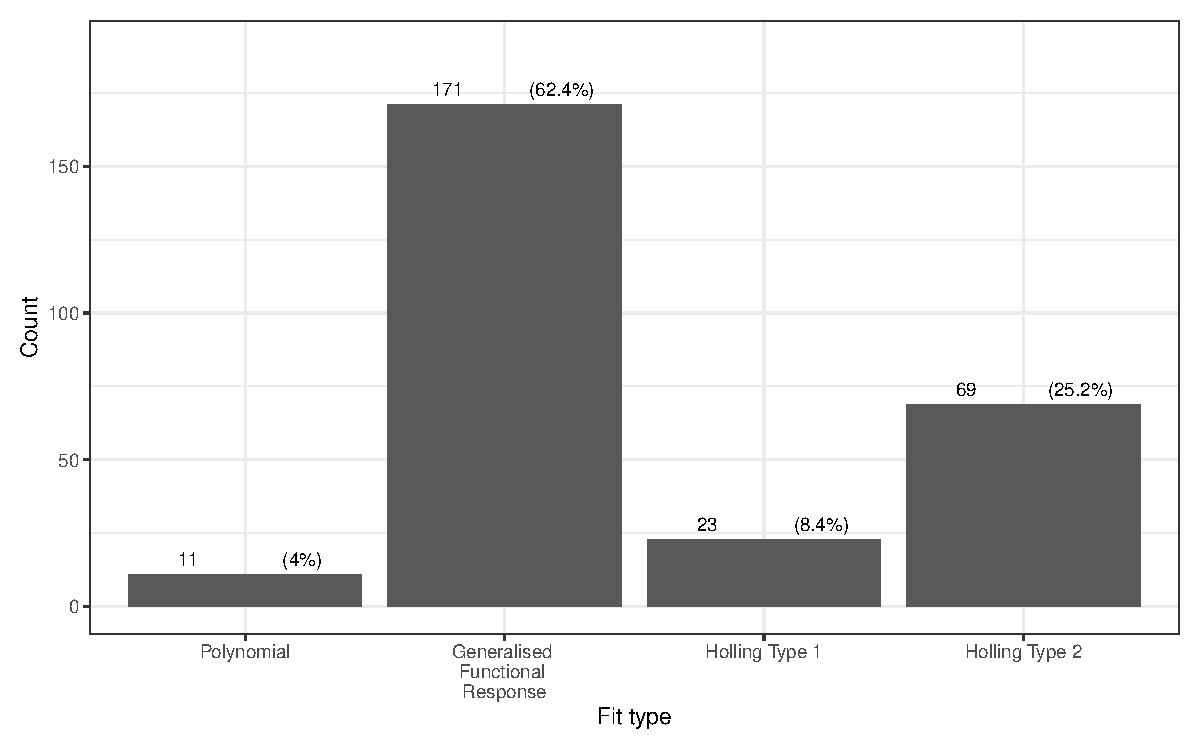
\includegraphics[width=1\textwidth]{../Results/Model_Comparison_Barchart.pdf}
	\caption{ID count by best fit model type}
\end{figure}

\subsection{Data subsets}

The dataset was preliminarily plotted in terms of eight factors: habitat, expermental conditions (lab/field/enclosure), consumer and rescoure thermal type, consumer and resource foraging movement and consumer and resource movement dimensionalty. All of these had a very similar ratio between the different best fits to that of the whole dataset, as can be seen from the four examples in Table 1. The few factors with slightly more varied proportions can be explained by the low quantity of data for that trait, for example passive resource foraging movement, which has only seven records. No particular trait was best fitted by a particular model, which is why the second focus of this paper is filter feeders. 

\begin{table}[ht!]
	\centering\csvreader[
	respect all,
	autotabular
	]{../Results/habitat_table.csv}{}{\csvlinetotablerow}
\end{table}

\begin{table}[ht!]
	\centering\csvreader[
	respect all,
	autotabular,
	]{../Results/labfield_table.csv}{}{\csvlinetotablerow}
\end{table}

\begin{table}[ht!]
	\centering\csvreader[
	respect all,
	autotabular
	]{../Results/res_movement_table.csv}{}{\csvlinetotablerow}
\end{table}

\begin{table}[ht!]
	\centering\csvreader[
	respect all,
	autotabular
	]{../Results/con_movement_table.csv}{}{\csvlinetotablerow}
	\caption{Different fit proportions in terms of various factors. The fit proportions shown by the overall data are shown at the bottom of each table.}
\end{table}

\subsection{Feeding mode}

Each of the IDs best fitted by a Holling type I response was allocated a feeding mode (either filter feeder or non-filter feeder), with the aim of exploring the 2004 claim by Jeschke et al.\parencite{Jeschke2004} that only filter feeders can display a Holling type I functional response. This allocation, along with the reference, can be seen in Table 2 and has been done according to the defintion of a filter feeder in the 2004 paper by Jeschke et al. This is a very broad definition that includes suspension feeders, trap builders, sediment filter feeders, those that only filter feed at certain stages in their lifecycle and also those that change feeding strategies according to prey abundance \parencite{Jeschke2004}.
From Table 2, it is apparent that a total of 11 of the 15 IDs best fit by a Holling type I functional response are classed as non-filter feeders.
This result is not insignifcant ($p < 2.2\times10^{-16}$ using G goodness of fit test). Figure 2 shows an example of a clearly linear functional response for a non-filter feeder consumer that is best fitted by the Holling type I equation.

\begin{table}[h!]
	\small
	\begin{tabular} {| l | l | l |}  \hline
		\textbf{ID} & \textbf{Taxa and Lifestage} & \textbf{Feeding Mode with Reference} \\ \hline
		695 & Stethorus punctum (Adult) & Non-Filter Feeder \parencite{Stethorus}  \\ \hline
		39839 & Rhyacophila dorsalis (Second Instar) &  Non-Filter Feeder \parencite{Rhyacophila}  \\ \hline
		39866 & Notonecta maculata (Fourth instar) & Non-Filter Feeder \parencite{Notonecta}  \\ \hline
		39890 & Anomalagrion hastatum  (Final Instar) &  Non-Filter Feeder \parencite{Anomalagrion}  \\ \hline
		39896, 39905 & Chaoborus americanus ( Fourth instar) & Non-Filter Feeder  \parencite{Chaoborus}  \\ \hline
		39920 & Ranatra dispar (Fifth instar)  &  Non-Filter Feeder \parencite{Ranatra}  \\ \hline
		40010 & Nereis (Hediste) diversicolor (Adult) & Filter Feeder \parencite{Nereis}  \\ \hline
		40019 & Parabroteas sarsi (Adult) & Filter Feeder \parencite{Copepod}  \\ \hline
		40026 &  Cyclops kolensis (Adult) & Non-Filter Feeder \parencite{Cyclops}  \\ \hline
		40066 & Praunus flexuosus (Adult) & Filter Feeder \parencite{Praunus}  \\ \hline
		40089, 40094, 40097 & Sander vitreus (Juvenile) &  Non-Filter Feeder \parencite{Sander}  \\ \hline
		400121 & Aurelia aurita (Juvenile) & Filter Feeder \parencite{Aurelia} \\ \hline
	\end{tabular}
	\caption{The consumers of functional responses best fit by a Holling Type I fit. Feeding mode has been based on the defintion used by Jeschke et al \parencite{Jeschke2004}}
\end{table}

\begin{figure}[ht!]
	\centering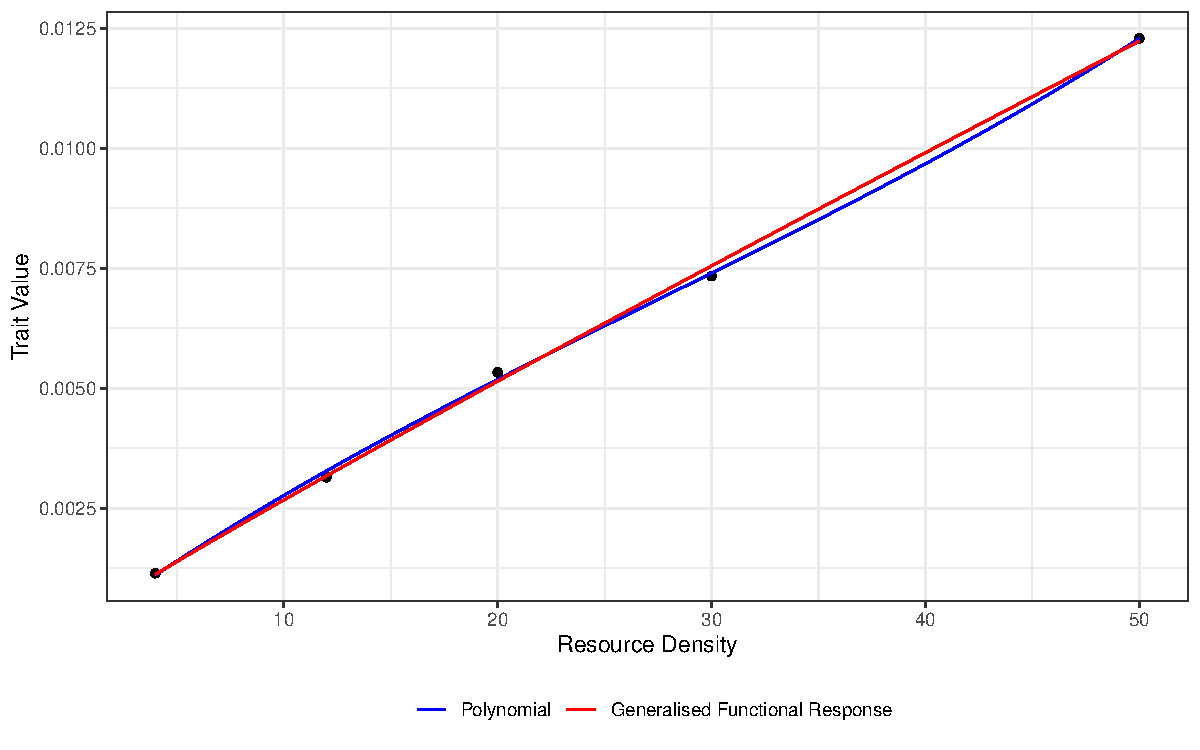
\includegraphics[width=1\textwidth]{../Results/Holling1_example.pdf}
	\caption{Functional response for a non-filter feeder consumer with Holling I best fit (ID = 39920, $q = -.0.055$, $h = 0$)}
\end{figure}


%%%%%%%%%%%%%%%% DISCUSSION %%%%%%%%%%%%%%%%


\section{Discussion}

\subsection{Mechanistic vs Phenomenological Models}

Functional response data are much better explained by the Holling mechanistic models than by a polynomial. This was to be expected, since the parameters in a polynomial do not correspond to biologically meaningful attributes and therefore have no underpinning scientific reasoning.
This is not to say that another mechanistic model might not describe the functional response with even more accuracy; however it does show the value of having models with a biological basis and provides evidence for their outperforming of phenomenological models.

\subsection{The Holling Type I Response}

The discrepancy between the expected and observed numbers of non-filter feeders with a type I functional response could be explained in two ways:

1) The limiting values of $a$ and $h$ used to subset the Holling type I response from the generalised functional response could have been inadequate, as they were not chosen using a mathematical method. As well as some functional responses being mis-classified as type I, some functional responses that should have been type I may have been missed.

2) Both Holling type II and III functional responses are linear away from the prey density limits. It is possible that not enough data were collected at very low and very high prey densities to display a type II or type III functional response, which is why they have been interpretted as type I.

Several different models have now been produced and  further work has been done to refine the Holling models, with modifications to account for both predator and prey size \parencite{Aljetlawi2004}, foraging dimensionality \parencite{Pawar2012} and changes over spatial scales \parencite{Rincon2017}, among others, all of which could impact the results of this study. The work by Seo and DeAngelis in describing the type I response shows a much more complicated dynamical system than formerly hypothesised \parencite{Seo2011}, which, if considered in this paper, could have provided evidence for the type I exclusivity to filter feeders. Many different models could further be applied to the empirical dataset to better understand the functional responses of both filter and non-filter feeders.

\subsection{The Holling Type II and Type III Responses}

Although not an interest of this paper, it is worth noting the high proportion of IDs with a type III response as the best fit, given that type II is considered to be the most common generally \parencite{Holling1959b}. This is most likely explained by the strict boundaries imposed between the two types. The fitting and tests done in this paper do not reflect the complexities of the two types or the overlaps that are commonly seen. If the plots of those IDs classed as type III are viewed, it can be seen that many better resemble a type II curve ( an example ID is shown in figure 3), suggesting further differentiation is needed than just setting $q\approx0$. This could be because this work has not taken into account intermediate functional responses, which may better explain much of the dataset than the pure repsonses \parencite{Jeschke2004}.

\begin{figure}[ht!]
	\centering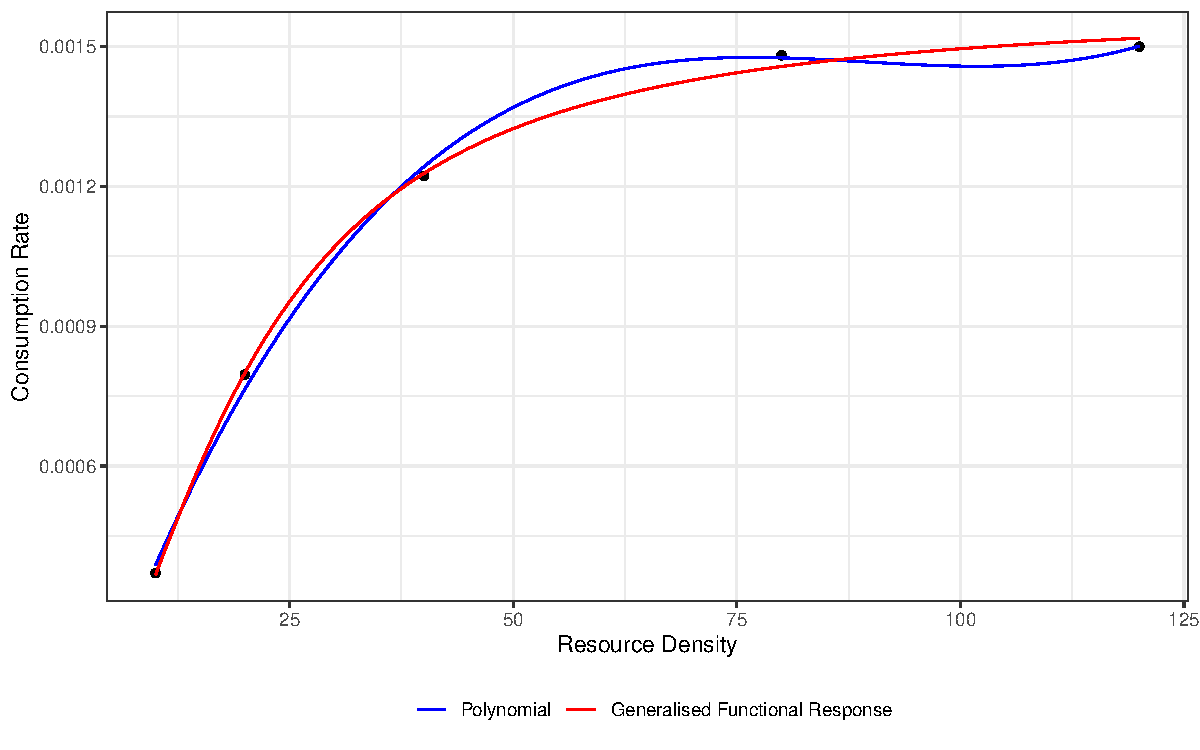
\includegraphics[width=1\textwidth]{../Results/GFR_Holling2_example.pdf}
	\caption{Holling Type II shape for a functional respnse best fit by a general functional response equation (ID = 39864, $q = 0.764$, $h = 632$)}
\end{figure}

\subsection{Concluding Remarks}

In the case of the Holling models and a polynomial, mechanistic models fit significantly better to an empirical dataset than phenomenological models. Although this might not be true for all mechanistic models as it depends on the accuracy of the model in describing nature, this is strong evidence for the superiority of mechanistic models over phenomenologial models.

Within the limits of the data provided, a Holling type I response is not exclusive to filter feeders, as has been previously suggested. However this may be due to a number of factors and so further research is required, perhaps using more sophisticated versions of Holling's models, to gain a more accurate picture.


\newpage
\printbibliography

\end{document}
